Using the reconstructed objects discussed in the previous chapter, 
we can select the Higgs events by selecting events with two leptons 
and \met. But, the selected events contain not only signal, 
but also backgrounds. A challege is that the production rate 
of the backgrounds is much larger than that of signal. 
\begin{figure}[htp] 
\centering 
\begin{tabular}{c} 
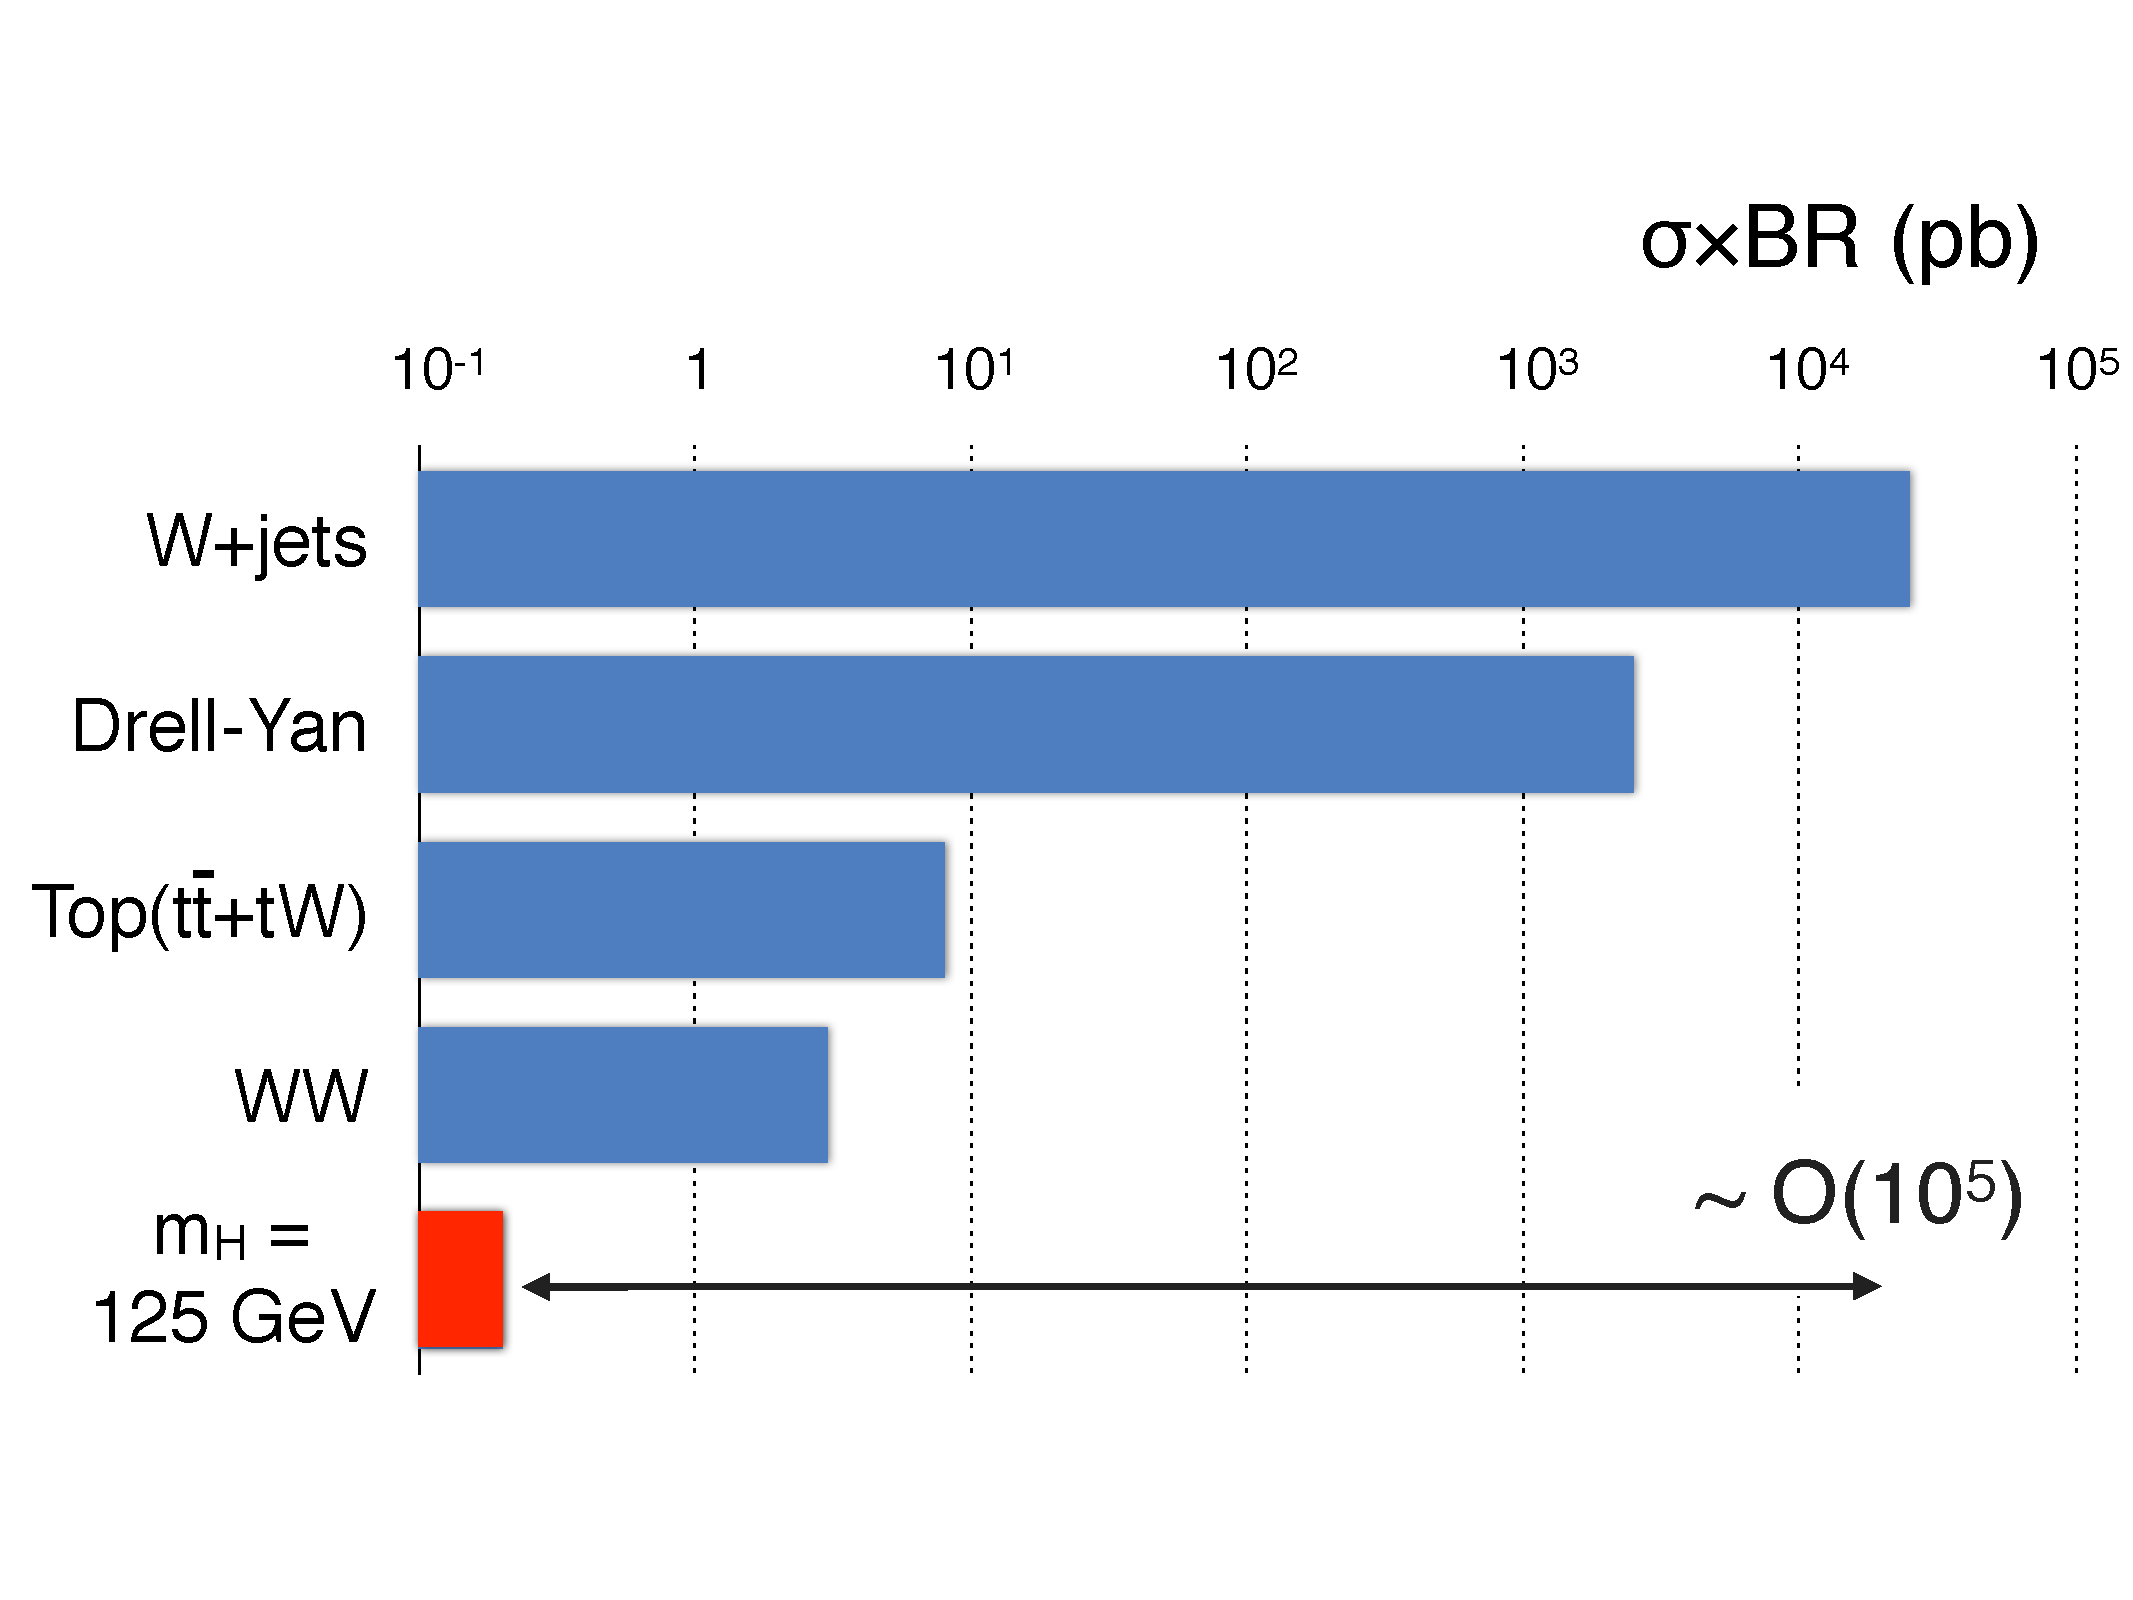
\includegraphics[width=0.95\textwidth]{figures/BkgProdRate.pdf} 
\end{tabular} 
\caption{The cross section $\times$
branching ratio($\sigma \times BR$) for the major background
processes and the SM \mHi=125~\GeV\ hypothesis.} 
\label{fig:bkgprodrate} 
\end{figure} 
Fig.~\ref{fig:bkgprodrate} shows the cross section $\times$ 
branching ratio($\sigma \times BR$) for the major background 
processes and the SM \mHi=125~\GeV\ hypothesis. 
The production rate of backgrounds is much larger than the signal. 
For example, the $\sigma \times BR$ of the \Wjets\ is a factor of 
$\mathcal{O}(10^5)$ larger than that of signal.  
Therefore, we need to apply stringent requirements which 
select the signal events with high efficiency, and suppress 
background events with a high rejection rate.  

The backgrounds can be divided into two categories depending on 
the way they can be suppressed. The first kind is reducible 
backgrounds which can be suppressed by tighting the requirements 
on the object selection. The other kind is irreducible backgrounds 
which have the exactly same final states as signal, 
therefore they can not be suppressed by tightening object selections,  
but by using event kinematics. 

This section describes the selection criteria to suppress the
reducible backgrounds. The requirements are imposed to 
trigger, vertex, electron, muon, jets, and top-tagging. 
In addition, there are additional requirements to suppress 
particular backgrounds. All these requirements are designed 
to select events containing a pair of Ws to make a subset of 
sample with a reasonable signal-to-background ratio for 
signal extraction. 


%%%%%%%%%%%%%%%%%%%%%%%%%%%%%%%%%%%%%%%%%%%%%%%%%%%%%%%%%%%%%%%%%%
\section{Trigger}

As seen in section~\ref{subsec:kinimetic_variables}, \hww{} events have trailing lepton 
whose transverse momentum goes down very low for low \mHi{} hypotheses. 
But, triggering low 
\pt{} leptons is very challenging because of large background events. 
Therefore, in order to record signal events with high efficiency, 
we need to trigger on the leading lepton, 
or on the both leptons. The option to trigger on the leading lepton 
is not possible because the identification 
and isolation requirements should be very tight, and momentum threshold should be very 
high to maintain a sustainable bandwidth. Thus, we trigger on the both leptons. 
The double-lepton triggers we designed for this analysis have high efficiency for  
signal events, but are loose enough to collect events in the several control regions 
we use for various studies. We also use control region triggers that allow 
fake rate and lepton selection efficiency measurements with a precision
good enough for this analysis. 

%\textcolor{red}{Where can I check the bandwidth of triggers? want to know 
%the total bandwidth of CMS and the bandwidth of triggers we use}

\subsection{Analysis Triggers}

The double-lepton triggers that are listed in Table~\ref{tab:trg_doublelepton} require 
two HLT objects, and each of them is required to match an L1 seed. The offline lepton \pt{} 
requirement is 20/10 \GeV, so the online lepton \pt{} reuquirement is a bit looser, 17/8 \GeV, 
in order to be avoid loosing events by online selection. In addition,
the longitudinal distance between the two vertices of the leptons is required 
to be less than 0.2~cm in order to suppress pileup events. 

For electron HLT objects there are additional requirements on
the shower shapes, %(H/E, $\sigma_{\eta\eta}$), 
the track-to-cluster matching and 
%($|\Delta\eta|$, $|\Delta\phi|$, $|\frac{1}{E}-\frac{1}{p}|$),
the track/calorimeter isolation. %(ECalIso, HCalIso, TrkIso). 
The exact variables and cut values are described in Table~\ref{tab:trg_requirement_def}.
In the table, the naming convention of CMS HLT triggers are shown 
with the corresponding requirements. 
The H/E is the ratio of energy deposit in HCAL to that of ECAL. 
The $\sigma_{\eta\eta}$ is the weighted sum of \Eta{} difference between the 
seed crystal and the 5x5 crystals surrouding it.   
The $|\Delta\eta|(|\Delta\phi|)$ is the difference in absolute value between 
the center of the supercluster and the direction of the track trajectory 
in \Eta($\phi$) direction.   
The $|\frac{1}{E}-\frac{1}{p}|$ is the difference between 
the reciprocal of supercluster energy 
and the reciprocal of the track momentum.  
The $\mathrm{ECalIso/E_T}$, $\mathrm{HCalIso/E_T}$ and $\mathrm{TrkIso/E_T}$ 
are the sum of the trasverse energy within $dR<0.3$ % \textcolor{red}{(checked)} 
around the center of the energy deposit or the track trajectory
divided by the transverse energy, $\mathrm{E_T}$. 
% E_T(SC) for Ecal, and elecand.pt() for Hcal and Tk (guess this is track momentum)  
Because online variables are constructed using more simplified algorithms 
than the offline variables, 
they do not exactly correspond to the offline ones. To account for this, we measure 
the trigger efficiency with respect to the offline selection, 
and apply corrections accordingly. 
The details on this can be found in~\ref{subsec:trg_eff} where the 
measurement on the trigger efficiency is discussed.
%\textcolor{red}{what is TkMu8? what is the iso requirement on single muon triggers?} 

\begin{table}[!ht]
  \centering 
  \begin{tabular} {l|l}
  \hline
  Double-lepton trigger name & L1 seed \\
  \hline \hline
  HLT\_Ele17\_CaloIdT\_CaloIsoVL\_TrkIdVL\_TrkIsoVL\_ 	    &  L1\_DoubleEG\_13\_7  \\
  Ele8\_CaloIdT\_CaloIsoVL\_TrkIdVL\_TrkIsoVL\_v[15-19] 	&                       \\ 
  %190456-190738 %190762-191419 %191512-194533
  \hline
  HLT\_Mu17\_Mu8\_v[16-22] 	    & L1\_DoubleMu\_10\_Open    \\ %190456-193686 %193806-194533
  HLT\_Mu17\_TkMu8\_v[9-14] 	& OR L1\_DoubleMu\_10\_3p5  \\ %190456-193686 %193806-194533
  \hline
  HLT\_Mu17\_Ele8\_CaloIdT\_CaloIsoVL\_ 	& L1\_Mu12\_EG7     \\
  TrkIdVL\_TrkIsoVL\_v[4-9] 	            &     \\
  %190456-190738 %190762-191419 %191512-193686 %193806-194533
  HLT\_Mu8\_Ele17\_CaloIdT\_CaloIsoVL\_	    & L1\_MuOpen\_EG12       \\ 
  TrkIdVL\_TrkIsoVL\_v[4-9] 	            & OR L1\_Mu3p5\_EG12     \\ 
  %190456-190738 %190762-191419 %191512-193686 %193806-194533
  \hline
  \end{tabular} 
  \caption{Double-lepton triggers used to collect signal events.} 
  \label{tab:trg_doublelepton}
\end{table}
%
\begin{table}[!ht]
  \centering 
  \begin{tabular} {l|l}
  \hline
  Single-lepton trigger name & L1 seed \\
  \hline \hline
  HLT\_Ele27\_WP80\_v[8-11] & L1\_SingleEG20 OR L1\_SingleEG22  \\ 
  %190456-190738 %190762-191419 %191512-194533
  \hline 
  HLT\_IsoMu24\_eta2p1\_v[11-15]   & L1\_SingleMu16er  \\  
  %190456-190738 %190762-193686 %193806-194533
  \hline \hline
  \end{tabular}
  \caption{Single-lepton triggers used to collect signal events.} 
  \label{tab:trg_singlelepton}
\end{table}

%
\begin{table}[!ht]
 \centering
 \begin{tabular}{l|c}
   \hline
   name                       &  criterion \\
   \hline \hline
   \multirow{2}{*}{CaloId\_T} & $\mathrm{H/E < 0.15 (0.10) }$ \\
                               & $\sigma_{\eta\eta}\mathrm{< 0.011\;(0.031)}$ \\
    \hline
   \multirow{2}{*}{CaloId\_VT} & $\mathrm{H/E < 0.05 (0.05) }$ \\
                               & $\sigma_{\eta\eta}\mathrm{< 0.011\;(0.031)}$  \\
    \hline \hline
    \multirow{2}{*}{TrkId\_VL} & $|\Delta\eta|\mathrm{< 0.01\; (0.01)}$ \\
                               & $|\Delta\phi|\mathrm{< 0.15\;(0.10)}$  \\
    \hline
    \multirow{2}{*}{TrkId\_T} & $|\Delta\eta|\mathrm{< 0.008\; (0.008)}$ \\
                              & $|\Delta\phi|\mathrm{< 0.07\;(0.05)}$ \\
    \hline \hline
    \multirow{2}{*}{CaloIso\_VL} & $\mathrm{ECalIso/E_T <0.2\;(0.2)}$ \\
                                 & $\mathrm{HCalIso/E_T <0.2\;(0.2)}$ \\
    \hline
    \multirow{2}{*}{CaloIso\_T} & $\mathrm{ECalIso/E_T <0.15\;(0.075)}$ \\
                                 & $\mathrm{HCalIso/E_T <0.15\;(0.075)}$ \\
    \hline
    \multirow{2}{*}{CaloIso\_VT} & $\mathrm{ECalIso/E_T <0.05\;(0.05)}$ \\
                                 & $\mathrm{HCalIso/E_T <0.05\;(0.05)}$ \\
    \hline \hline
    TrkIso\_VL                   & $\mathrm{TrkIso/E_T <0.2\;(0.2)}$ \\
    \hline
    TrkIso\_T                   & $\mathrm{TrkIso/E_T <0.15\;(0.075)}$ \\
    \hline
    TrkIso\_VT                   & $\mathrm{TrkIso/E_T <0.05\;(0.05)}$ \\
    \hline \hline
    \multirow{8}{*}{WP80} 		& $\mathrm{H/E < 0.10 (0.05) }$ \\
                               	& $\sigma_{\eta\eta}\mathrm{< 0.01\;(0.03)}$ \\
    							& $|\Delta\eta|\mathrm{< 0.007\; (0.007)}$ \\
                               	& $|\Delta\phi|\mathrm{< 0.06\;(0.03)}$  \\
                               	& $|\frac{1}{E}-\frac{1}{p}|\mathrm{< 0.05\;(0.05)}$  \\
    							& $\mathrm{ECalIso/E_T <0.15\;(0.10)}$ \\
                                & $\mathrm{HCalIso/E_T <0.10\;(0.10)}$ \\
                       			& $\mathrm{TrkIso/E_T <0.05\;(0.05)}$\\
    \hline
 \end{tabular}
 \caption{Summary of requirements applied to electrons in the analysis triggers.
The selection requirements are shown for electrons in the barrel (endcap).
The abbrevation in the names means L=Loose, VL=Very Loose, T=Tight, and VT=Very Tight.}
 \label{tab:trg_requirement_def}
\end{table}

\subsection{Utility Triggers}

The efficiency measurements of the lepton selection requirements 
are performed using the \tnp{} method~\cite{} on \dyll{} events. 
In order to use \tnp{} method, we should select a pure sample 
of \dyll{} events to reduce bias due to selecting non-prompt leptons from 
other background processes or pileup. Apart from the analysis triggers, for this 
measurement we do not have to select all available events, but a pure sample with 
an adequate statistics. The single lepton triggers used to collect signal events, 
listed in Table~\ref{tab:trg_singlelepton}, also can be used to select 
\dyll{} events. The leading lepton is likely to be triggered, making the 
trailing lepton unbiased sample that covers a wide range of 
kinematic region that streches to the low lepton \pt.   

In order to estimate jet-induced backgrounds such as \Wjets{} that have a non-prompt 
lepton that passes the full lepton selection, we use "fake rate" method.  
The details of this method are discussed in~\ref{sec:wjets}. 
In this method we define a loose lepton selection, and calculate the ratio
, fake rate, of the 
events that pass the full selection to the events that pass the loose 
selection, using a data sample of single-lepton events dominated by QCD processes. 
The fake rate differs by event kinematics
such as \pt{} and \Eta{} of the lepton, and the \pt{} of the leading jet 
that recoils off the lepton. Because the leptons in the data sample
collected by the analysis triggers are trigger objects, the loosest possible 
``loose" definition is the trigger requirement of the analysis triggers.
We devised a set of single-lepton triggers that have a loose or the same requirements 
on leptons as the double-lepton triggers. 
%Note that the single lepton triggers have tighter requirements on leptons. 
In order to cover large lepton \pt{} range, 
we use several triggers with different lepton \pt{} thresholds.
Because the jet \pt{} distribution is exponentially falling, 
we need triggers that require corrected leading jet \pt{} be greater than 30 \GeV. 
These triggers give sufficient samples for systematic study on the fake rate method. 

%For the data-driven estimation for \dyll{} backgrounds we have alternate method 
%that uses photon + jets events. These events are triggered by photon triggers 
%and the photon triggers used for this analysis are listed in the Table~\ref{tab:}.


\begin{table}[!ht]
  \begin{center}
 {\small
  \begin{tabular} {l|l}
\hline
 Trigger name & L1 seed \\
\hline\hline
 HLT\_Ele8\_CaloIdT\_TrkIdVL\_v[2-5]	& L1\_SingleEG5 		\\ %190456-190738 %190762-191419 %191512-194533
 HLT\_Ele8\_CaloIdT\_CaloIsoVL\_		& L1\_SingleEG7 		\\ 
 TrkIdVL\_TrkIsoVL\_v[12-15]			&  						\\ %190456-190738 %190762-191419 %191512-194533
 HLT\_Ele17\_CaloIdT\_CaloIsoVL\_  		& L1\_SingleEG12		\\ 
 TrkIdVL\_TrkIsoVL\_v[3-6]  			& 						\\ %190456-190738 %190762-191419 %191512-194533
 HLT\_Ele8\_CaloIdT\_CaloIsoVL\_      	& L1\_SingleEG7         \\
 TrkIdVL\_TrkIsoVL\_Jet30\_v[3-7]      	& 						\\ %190456-190738 %190762-191419 %191512-194533
 HLT\_Ele17\_CaloIdT\_CaloIsoVL\_		& L1\_SingleEG12		\\ 
 TrkIdVL\_TrkIsoVL\_Jet30\_v[3-7]		& 						\\ %190456-190738 %190762-191419 %191512-194533
	\hline \hline
 HLT\_Mu8\_v[16-18] 	&  L1\_SingleMu3  		\\ %190456 - 194533
 HLT\_Mu17\_v[3-5]      &  L1\_SingleMu12   	\\ %190456 - 194533   
%	\hline \hline
% HLT\_Photon22\_R9Id90\_HE10\_Iso40\_EBOnly\_v[2-4]					& L1\_SingleEG22		\\ %190456-190738 190762-191419 %191512-194731
% HLT\_Photon36\_R9Id90\_HE10\_Iso40\_EBOnly\_v[2-4]					& L1\_SingleEG22		\\ %190456-190738 190762-191419 %191512-194731
% HLT\_Photon50\_R9Id90\_HE10\_Iso40\_EBOnly\_v[2-4]					& L1\_SingleEG22		\\ %190456-190738 190762-191419 %191512-194731
% HLT\_Photon75\_R9Id90\_HE10\_Iso40\_EBOnly\_v[2-4]					& L1\_SingleEG22		\\ %190456-190738 190762-191419 %191512-194731
% HLT\_Photon90\_R9Id90\_HE10\_Iso40\_EBOnly\_v[2-4]					& L1\_SingleEG22		\\ %190456-190738 190762-191419 %191512-194731
    \hline 
  \end{tabular}
}
  \caption{Utility triggers for fake rate method. %and zeta method. 
  The identification and isolation requirements for electrons are described in Table~\ref{tab:trg_requirement_def}.
%The identification and isolation requirements for photons are described in Table~\ref{tab:PhotonPlusLeptonTriggerCuts}.
}
%and ``$\zeta$ method " are used for Drell-Yan background estimation.}
   \label{tab:triggers_util}
  \end{center}
\end{table}

%
%\begin{table}[htb]
%  \centering
%  \begin{tabular}{l|c}
%    \hline
%    name                        &  criterion \\
%    \hline \hline 
%    \multirow{1}{*}{R9Id90} 	& $\mathrm{R9 > 0.9 }$ \\
%    \hline 
%    \multirow{1}{*}{HE10} 		& $\mathrm{H/E < 0.1 }$ \\
%    \hline 
%    \multirow{3}{*}{Iso40}     	& $\mathrm{ECalIso} < 4.0 $ \\
%                                & $\mathrm{HCalIso} < 4.0 $ \\
%                                & $\mathrm{TrkIso}  < 4.0 $ \\
%    \hline 
%  \end{tabular}
%   \caption{Summary of requirements applied in the photon triggers used for this analysis.}
%   \label{tab:trg_requirement_def_photon}
%\end{table}

%%%%%%%%%%%%%%%%%%%%%%%%%%%%%%%%%%%%%%%%%%%%%%%%%%%%%%%%%%%%%%%%%%
\section{ Event Primary Vertex }
%\begin{itemize}
%\item \textcolor{red}{Track reconstruction : Kalman Filter, ...}
%\item \textcolor{red}{Vertex reconstruction : vertex finding, vertex fitting, ...}
%\item \textcolor{red}{Primary Vertex selection}
%\end{itemize}

The offline primary vertices are required to be within 24~\cm\ from the center of the 
detector%\textcolor{red}{(or beamspot?)} 
in z direction. 
It should be within 2~\cm\ from the beamspot in the radial direction. 
The degrees of freedom of the vertex fit should be 4 or larger. 
%\textcolor{red}{what does this mean exactly?} 

At high luminosity collisions, there are multiple proton-proton interactions 
in the same bunch crossing. In those interactions there is usually 
only one interaction that is of interest for our analysis, which triggered that event. 
These interactions tend to be associated with energetic objects, 
while the other interactions are mostly inelastic scatterings that produce soft objects.
Therefore, we choose the event primary vertex by selecting the primary vertex 
with the largest scalar sum of $\pt^2$ of tracks associated with the vertex. 
%The vertices of leptons are required to be very close to the event primary vertex.  



%%%%%%%%%%%%%%%%%%%%%%%%%%%%%%%%%%%%%%%%%%%%%%%%%%%%%%%%%%%%%%%%%%
\section{ Electron }
%\begin{itemize}
%\item \textcolor{red}{Electron reconstruction : GSF track, seeding, ... }
%\item \textcolor{red}{ID  : MVA (list of input variables, trainig samples, cut values)}
%\item \textcolor{red}{ISO : list of variables to calculate the final cut variable, cut values  }
%\end{itemize}

An electron candidate is reconstructed if there is a track and a supercluster energy 
deposit compatible with the track momentum. There are multiple sources of 
electrons which do not originate from hard interactions. These electrons 
are called ``non-prompt electrons" as opposed to the 
``prompt electrons" originated from hard interactions. 
Of these, electrons that is originated from jets is called ``fake electrons or fakes".
We can get fake electrons if  
\begin{itemize}
\item $\pi^0$ decays to two photons, and one of the two photons
      undergoes an asymmetric conversion to an electron-positron pair, \textit{i.e.}, 
      one of the them carries most of the photon momentum. 
\item $\pi^\pm$ is converted to $\pi^0$ in the ECAL(charge exchange process), 
      and the $\pi^0$ decays to a pair of photons.
\item B or D meson decays semi-leptonically.  
\end{itemize}
In order to suppress fake electrons, we apply selections composed of 
requirements on the identification,
%(track-to-supercluster matching, 
%track fit quality, shower shape, energy loss due to \brem\, ratio of hadronic energy
%to electromagnetic energy), 
isolation and impact parameter.  
Other source of non-prompt electrons is a photon conversion 
to a pair of electron and a positron 
in the material. If the conversion is asymmetric, \textit{i.e.} one particle carries 
most of the photon momentum, that particle can be selected as an electron 
candidate. Thus, we apply additional requirement on the convertion rejection.

% indentification 
For the electron identification we use a BDT-based multivariate 
approach~\cite{Chatrchyan:2012ufa}. The Boosted Decision Tree(BDT)~\cite{Hocker:2007ht} 
is a multivariate algorithm that uses distributions of multiple variables 
and their correlations to optimally distinguish one hypothesis from the other.  
The trainig is done with 2011 data; \dyll{} events for signal and QCD-dominated events 
collected by the fake rate triggers listed in section~\ref{sec:trigger}. 
In order to increase the separation, and to mitigate a possible bias 
due to the trigger selections, a set of preselection cuts that are as tight as the trigger 
requirements is applied as follows :  
\begin{itemize}
  \item $\pt>10~\GeV$ and $|\eta| < 2.5$
  \item $\sigma_{i\eta i\eta} < 0.01/0.03$ (barrel/endcap)
  \item $|\Delta\phi_{in}| < 0.15/0.10$ (barrel/endcap)
  \item $|\Delta\eta_{in}| < 0.007/0.009$ (barrel/endcap)
  \item $\textrm{H/E}< 0.12/0.10$ (barrel/endcap)
  \item $\displaystyle \frac{\sum_{\textrm{tracks with dR}<0.3}\Et}{\pt}<0.2$
  \item $\displaystyle \frac{\left(\sum_{\textrm{ECAL with dR}<0.3}\Et\right)-1}{\pt}<0.2$
  \item $\displaystyle \frac{\sum_{\textrm{HCAL with dR}<0.3}\Et}{\pt}<0.2$
\end{itemize}
%The additional subtraction of 1 GeV in the numerator of ECAL isolation is 
%to suppress the constant noise. 
The input variables to the MVA are the following.
\begin{itemize}
\item kinematics : $\pt$,  $\eta$
\item shower shape : $\sigma_{i\eta i\eta}$, $\phi_{i\eta i\eta}$, $\Delta \phi_{SC}$, $\Delta \eta_{SC}$, $E_{3\times3}/E_{5\times5}$(R9), $E_{1\times5}/E_{5\times5}$
\item track fit quality : $\chi^2(\textrm{GSF})/\textrm{ndof} $, $\chi^2(\textrm{CTF})/\textrm{ndof}$ 
\item $\textrm{N}_\textrm{layers}$  
\item cluter-track matching (geometry) : $\Delta \phi_{in}$, $\Delta \eta_{in}$, $\Delta \eta_{out}$
\item cluter-track matching (energy-momentum) : $E_{SC}/p$, $E_{C}/p_{out}$, $1/E_\textrm{SC} - 1/p$ 
\item fraction of energy carried away by \brem{} : $f_{brem}$ 
\item ratio of hadronic energy to EM energy  : $H/E$ 
\item impact parameter :  transverse and 3D impact parameters w.r.t. primary vertex
\item $E_{\textrm{PS}}/E_{\textrm{SC}}$
\end{itemize}
The $\sigma_{i\eta i\eta}$($\phi_{i\eta i\eta}$) is the weighted sum of \Eta($\phi$) 
difference between the seed crystal which contains the highest energy, 
and the $5\times5$ crystals surrouding it.
The $\Delta \phi_{SC}$($\Delta \eta_{SC}$) is the width of average distance 
between the seed crystal and the $5\times5$ crystals surrouding it.
The $E_{3\times3}/E_{5\times5}$(R9) and $E_{1\times5}/E_{5\times5}$ 
are the ratio of energy deposit in the $3\times3$($1\times5$) crystals to the
$5\times5$ crystals centered at the seed crystal. 
The $\chi^2(\textrm{GSF})/\textrm{ndof}$ and $\chi^2(\textrm{CTF})/\textrm{ndof}$
are the variables to measure the quality of GSF and CTF track fits, respectively. 
$\textrm{N}_\textrm{layers}$ is the number of tracker layers 
where the electron made hits. 
The $\Delta \phi_{in}$($\Delta \eta_{in}$) is the distance in \Eta($\phi$) direction 
between the supercluster position and the track trajectory extrapolated from 
the interaction pointto the supercluster. 
$\Delta \eta_{out}$ is the distance in \Eta{} direction
between the supercluster position and the track trajectory extrapolated 
from the supercluster to the interaction point.
The $E_{SC}/p$ is the supercluster energy divided by the track momentum 
at the point of closest approach (PCA) to the beam spot.
The $E_C/p_{out}$ is the electron cluster energy divided by the track momentum 
at the PCA to the electron cluster, extrapolated from the outermost track state. 
The $1/E_\textrm{SC} - 1/p$ is the difference between the reciprocals 
of the supercluster energy and the track momentum.
The $f_{brem}$ is the ratio of the difference between the momemta measured 
at the vertex and the outermost state to the momemtum measured at the 
vertex. This variable shows the fraction of momentum loss by \brem. 
The H/E is the ratio of the energy deposit in the HCAL tower behind the electromagnetic 
seed cluster to the energy of the seed cluster.
The $E_{\textrm{PS}}/E_{\textrm{SC}}$ is the ratio of the energy deposit in the preshower 
detector and the energy deposit in the supercluster. 
\begin{table}[!ht]
  \centering 
  \begin{tabular} {c||c|c|c}
  \hline
        & $0<|\eta|<0.8$ & $0.8<|\eta|<1.479$ & $1.479<|\eta|<2.5$\\
  \hline \hline
   $10~\GeV<\pt<20~\GeV$    & 0.0   & 0.1   & 0.62 \\ 
  \hline
   $\pt>20~\GeV$            & 0.94  & 0.85  & 0.92 \\ 
  \hline 
  \end{tabular}
  \caption{Cut values on BDT output for electron identification. Electrons with BDT output
  greater than the corresponding values in the table are considered as good electrons.} 
  \label{tab:electronid_bdtcut}
\end{table}
For selecting good electrons, we finally require that the BDT score be greater 
than the values depending on the kinematic region as shown in Table~\ref{tab:electronid_bdtcut}. 

% isolation 
The isolation requirements are imposed by computing isolation variable using 
PF candidates. 
In the high luminosity environment there are random contribution from pileup 
to the isolation calculation, so we need to correct for this to prevent 
a degradation of the isolation requirement. 
To reduce the contributions from the random charged PF candidates, they are 
required to be close to the event primary vertex. The contribution from 
the random neutral PF candidates is corrected by subracting the expected contribution. 
The variable is defined as a scalar sum of the \pt{} of the 
PF candidates satisfying the following requirements. 
\begin{itemize}
\item $\Delta R~<~0.4$ to the electron in the $\eta \times \phi$ plane
\item Other PF electrons and PF muons in the isolation cone are vetoed
\item Gamma PF candidates are required to be outside of the footprint 
      veto region of $\Delta R~<~0.08$ 
\item Charged hadron PF candidates are required to be outside of the footprint 
      veto regoin of $\Delta R~<~0.015$ 
\item Charged hadron PF candiates are required to be associated 
      with the event primary vertex : their closest vertex should be the 
      event primary vertex
\item Neutral components are corrected by subtracting pileup contribution which is 
      calculated by $\rho \times \textrm{A}_{\rm{eff}}$,
\end{itemize}
where $\rho$ is the event-by-event energy density~\cite{} calculated using 
\texttt{kt6PFJets} algorithm~\cite{}, 
and $\textrm{A}_{\textrm{eff}}$ is the effective area shown in Table~\ref{tab:electron_Aeff}. 
\begin{table}[!ht]
  \centering 
  \begin{tabular} {c||c|c|c|c|c|c}
  \hline
    $|\eta|$    & 0 - 1.0 & 1.0 - 1.479 & 1.479 - 2.0 & 2.0 - 2.2 & 2.2 - 2.3 & 2.3 - 2.4  \\
  \hline \hline
    $\textrm{A}_{\rm{eff}}$  & 0.19 & 0.25 & 0.12 & 0.21 & 0.27 & 0.44 \\ 
  \hline 
  \end{tabular}
  \caption{Effective area used for electron isolation calculation.}
  \label{tab:electron_Aeff}
\end{table}

The isolation variable we cut on is calculated as 
\begin{equation}
\frac{\rm{Iso}_{PF}}{\pt}
=
\left[ \rm{Iso}_{charged \, hadron} + \left\{ \rm{Iso}_{gamma} 
       + \rm{Iso}_{neutral \, hadron} -\rho \times \textrm{A}_{\textrm{eff}} \right\} \right]
\times \frac{1}{\pt}
\end{equation}
where $\rm{Iso}_{charged \, hadron}$, $\rm{Iso}_{gamma}$, and $\rm{Iso}_{neutral \, hadron}$ 
are the scalar sum of the \pt{} of the charged hadron, gamma and neutral hadron PF candidates, 
respectivlely, in the isolation cone of $0.4$ around the electron.
We require $\frac{\rm{Iso}_{PF}}{\pt}$ to be less than $0.15$ in both barrel and endcap.  

% conversion
In order to reject the electrons from a conversion from a photon, we reject the electron 
if there is a recontructed conversion vertex where one of the two tracks match with 
the electron, if the probability of the conversion vertex fit is greater than $10^{-6}$, 
if the distance between the conversion vertex and the point of closest approach 
to the event primary vertex is greater than 2~\cm,
and there is any missing hit in the electron track before the conversion vertex.   

% impact parameters
The impact parameter requirements are such that the transverse(longitudinal) impact parameter
between the electron track and the event primary vertex is less than 0.02 cm(0.1 cm). 

The efficiency of the full electron selection measured with 20/10~\GeV\ requirement 
in MC is about 80~\% for electrons in the \mHi=125~\GeV\ events 
and about 5~\% for electrons whose mothers are not Ws in W+jets.

%%%%%%%%%%%%%%%%%%%%%%%%%%%%%%%%%%%%%%%%%%%%%%%%%%%%%%%%%%%%%%%%%%
\section{ Muon }
%\begin{itemize}
%\item \textcolor{red}{Muon reconstruction : ...}
%\item \textcolor{red}{ID  : list variables and cut values }
%\item \textcolor{red}{ISO : MVA (list of input variables, trainig samples, cut values) }
%\end{itemize}

A muon candidate is reconstructed if there 
is a track in the tracker and/or are segments in the muon system. 
There are multiple sources of muons which do not originate from gauge boson decays. 
\begin{itemize}
\item decay-in-flight : a charged meson decays to muon in the tracker, 
\item punch-through : a charged meson survive the HCAL, and leaves 
\item B or D meson decays semi-leptonically.  
\end{itemize}
In order to reject muons from these sources, 
we apply a muon selection which is composed of requirements 
on the identification,
%(track fit quality, momentum resolution, 
%number of hits/segments in the tracker/muon system,  
%rejection of ), 
isolation and impact parameter.  

%identification
The identification requirements are as follows. 
\begin{itemize}
\item The muon should be identified as PF muon 
\item $\pt>10~\GeV$ and $|\eta|<2.4$ 
\item $N_{\textrm{track layers}}>5$ 
\item $N_{\textrm{pixel hits}}$
\item $\displaystyle \frac{\delta \pt}{\pt} < 0.1$  
\item $\displaystyle \frac{\chi^2_{\textrm{kink finder}}}{\textrm{ndof}} < 20$
\item The muon should be global muon or tracker muons  
\end{itemize}
where $N_{\textrm{layers}}$ is the number of tracker layers where the muon track made hits, 
the $N_{\textrm{pixel hits}}$ is the number of pixel hits of the muon track,
the $\displaystyle \frac{\delta \pt}{\pt}$ is the relative resolution 
of the muon \pt, 
and $\displaystyle \chi^2_{\textrm{kink finder}}/\textrm{ndof}$ is the quality 
of kink finder algorithm which finds muons from decay-in-flights.  
In addtion to these requirements, the muons are required to be the global muons with 
$\chi^2/\textrm{ndof}$ of the the global fit less than 10, 
at least one muon hit matching the global fit 
%\textcolor{red}{(what is the difference between hits and segments?)},  
and having at least two muon segments in different muon stations. 
If the moun is not a global muon, it can be a tracker muon satisfying that at least two muon 
segments one of which is in the outermost muon station are matched.  

%isolation 
For the isolation requirement, the MVA-based isolation variable~\cite{MuonRingIso} is used.
%to reduce contamination from non-isolated muons originating from jets. 
It uses the energy deposits of PF candidates of three categories, 
charged hadron, gamma and neutral hadrons in the concentric isolation cones
of size $\Delta R = 0-0.1,~0.1-0.2,~0.2-0.3,~0.3-0.4$ and $0.4-0.5$.
Neutral components are corrected by subtracting the pileup contribution which is 
calculated by $\rho \times \textrm{A}_{\textrm{eff}}$ where $\rho$ (\texttt{kt6PFJets}) is the 
event-by-event energy density and $\textrm{A}_{\textrm{eff}}$ is the effective area.  
Effective areas are from Fall 11 simulation (\texttt{kMuEAFall11MC}), and 
values are shown in Table~\ref{tab:muAeff}.  
Exact definition of input variables to the MVA is the following :
\begin{itemize}
\item PF charged hadron
	\begin{itemize}
    \item minimum of $\textrm{Iso}_\textrm{PF charged, 01}/\pt$ and 2.5	
    \item minimum of $\textrm{Iso}_\textrm{PF charged, 12}/\pt$ and 2.5	
    \item minimum of $\textrm{Iso}_\textrm{PF charged, 23}/\pt$ and 2.5	
    \item minimum of $\textrm{Iso}_\textrm{PF charged, 34}/\pt$ and 2.5	
    \item minimum of $\textrm{Iso}_\textrm{PF charged, 45}/\pt$ and 2.5	
	\end{itemize}
\item PF gamma : If negative, 0.0 is assigned
	\begin{itemize}
    \item minimum of $\left[\textrm{Iso}_\textrm{PF gamma, 01} - \rho \times \textrm{A}_{\textrm{eff}}\right]/\pt$ and 2.5 
    \item minimum of $\left[\textrm{Iso}_\textrm{PF gamma, 12} - \rho \times \textrm{A}_{\textrm{eff}}\right]/\pt$ and 2.5 
    \item minimum of $\left[\textrm{Iso}_\textrm{PF gamma, 23} - \rho \times \textrm{A}_{\textrm{eff}}\right]/\pt$ and 2.5 
    \item minimum of $\left[\textrm{Iso}_\textrm{PF gamma, 34} - \rho \times \textrm{A}_{\textrm{eff}}\right]/\pt$ and 2.5 
    \item minimum of $\left[\textrm{Iso}_\textrm{PF gamma, 45} - \rho \times \textrm{A}_{\textrm{eff}}\right]/\pt$ and 2.5 
	\end{itemize}
\item PF neutral hadron : If negative, 0.0 is assigned
	\begin{itemize}
    \item minimum of $\left[\textrm{Iso}_\textrm{PF neutral, 01} - \rho \times \textrm{A}_{\textrm{eff}}\right]/\pt$ and 2.5 
    \item minimum of $\left[\textrm{Iso}_\textrm{PF neutral, 12} - \rho \times \textrm{A}_{\textrm{eff}}\right]/\pt$ and 2.5 
    \item minimum of $\left[\textrm{Iso}_\textrm{PF neutral, 23} - \rho \times \textrm{A}_{\textrm{eff}}\right]/\pt$ and 2.5 
    \item minimum of $\left[\textrm{Iso}_\textrm{PF neutral, 34} - \rho \times \textrm{A}_{\textrm{eff}}\right]/\pt$ and 2.5 
    \item minimum of $\left[\textrm{Iso}_\textrm{PF neutral, 45} - \rho \times \textrm{A}_{\textrm{eff}}\right]/\pt$ and 2.5 
	\end{itemize}
\end{itemize}
where we define 
\begin{eqnarray} 
\textrm{Iso}_\textrm{PF,XY} 
= 
\sum_{
\begin{subarray}{l}
\textrm{PF candidates in the cone of} \\
\textrm{0.X}   < \Delta R^{\mu-\textrm{PF candidate}} < \textrm{0.Y} 
    \end{subarray} }
\pt
%\textrm{the scalar sum of \pt\ of PF candidates in the cone of 0.X} 
%< \Delta R^{\mu-\textrm{PF candidate}} < \textrm{0.Y}.
\end{eqnarray} 

We require that the MVA output be greater than 0.82 (0.86) in $10<\pt~<20~\GeV$ 
and 0.86 (0.82) in $\pt~>20~\GeV$. The cut values correspond to the ones in barrel (endcap).

\begin{table}[htp]
	\centering
		\begin{tabular}{c|c|c|c|c|c|c}
			\hline 
				\multicolumn{7}{c}{PF gamma} \\
	  	    \hline
			 	$|\eta|$     & $0.0 - 1.0$ & $1.0 - 1.479$ & $1.479 - 2.0$ & $2.0 - 2.2$ & $2.2 - 2.3$ & $2.3-$ \\       		
	  	    \hline \hline
				$0.0<dR<0.1$ & 0.004& 0.002& 0.003& 0.009& 0.003& 0.011 \\
				$0.1<dR<0.2$ & 0.012& 0.008& 0.006& 0.012& 0.019& 0.024 \\
				$0.2<dR<0.3$ & 0.026& 0.020& 0.012& 0.022& 0.027& 0.034 \\
				$0.3<dR<0.4$ & 0.042& 0.033& 0.022& 0.036& 0.059& 0.068 \\
				$0.4<dR<0.5$ & 0.060& 0.043& 0.036& 0.055& 0.092& 0.115 \\
	  	    \hline \hline 
				\multicolumn{7}{c}{PF neutral hadron} \\
	  	    \hline 
			 	$|\eta|$     & $0.0 - 1.0$ & $1.0 - 1.479$ & $1.479 - 2.0$ & $2.0 - 2.2$ & $2.2 - 2.3$ & $2.3-$ \\       		
	  	    \hline \hline
				$0.0<dR<0.1$ & 0.002& 0.004& 0.004& 0.004& 0.010& 0.014 \\
			    $0.1<dR<0.2$ & 0.005& 0.007& 0.009& 0.009& 0.015& 0.017 \\
			    $0.2<dR<0.3$ & 0.009& 0.015& 0.016& 0.018& 0.022& 0.026 \\ 
				$0.3<dR<0.4$ & 0.013& 0.021& 0.026& 0.032& 0.037& 0.042 \\ 
				$0.4<dR<0.5$ & 0.017& 0.026& 0.035& 0.046& 0.063& 0.135 \\ 
			\hline
		\end{tabular}
		\caption{ Effective areas used for muon isolation. They were calculated with Fall11 MC sample.}
	\label{tab:muAeff}
\end{table}

%impact parameter 
In addtion, we require transverse/longditudinal impact parameters 
to be associated with the event primary vertex. 
The transverse impact parameter is required 
to be less than 0.01 cm for $\pt<20~\GeV$ and 0.02 cm for $\pt>20~\GeV$. 
The longitudinal impact parameter is required to be less than 0.01 cm. 

The efficiency of the full muon selection measured with 20/10~\GeV\ requirement 
in MC is about 90~\% for muons in the \mHi=125~\GeV\ events 
and about 11~\% for muons whose mothers are not Ws in W+jets.

%%%%%%%%%%%%%%%%%%%%%%%%%%%%%%%%%%%%%%%%%%%%%%%%%%%%%%%%%%%%%%%%%%
\section{ Jet }
\label{sec:jetselection}
%\begin{itemize}
%\item \textcolor{red}{Jet reconstruction : anti-kT (dR = 0.5) }
%\item \textcolor{red}{Jet energy correction : L1Fastjet/L2/L3 (+ Residual correction in data) }
%\item \textcolor{red}{lepton veto ($dR>0.3$) }
%\item \textcolor{red}{MVA jet ID(list of input variables, training samples, cut values)}
%\item \textcolor{red}{two definitions : (1) jet bin counting($\pt>30~\GeV$) (2) top veto($10<\pt<30~\GeV$) }
% have a plot like this for MVA Jet ID? not sure how I drew this though
% maybe a script is somewhere on uaf
%http://uaf-2.t2.ucsd.edu/~jaehyeok/HWW/PhilJetIDMVA/dev/PhilJetIDMVAefssssssss.pdf
%\end{itemize}

In this analysis jets are selected by rejecting overlaps with selected electrons 
and muons. If the $\Delta R$ between a lepton and the jet is less than 0.3, the jet 
is likely to be a lepton, thus it is not considered as a jet. In the high pileup environment, 
clustering random PF particles from pileup interactions can lead to high \pt\ jets. 
To suppress this, we apply a BDT-based techique to suppress jets originated from pileups. 
The jets from pileup tend to be soft, so they need to be overlaid to pass the jet \pt\ threshold. 
Therefore, the energy deposit of the pileup jets are more spread 
than the ones from hard interactions. The following variables are used 
in the BDT-based suppression technique.
\begin{itemize}
\item Number of reconstructed primary vertices in the event
\item Kinematics of the jet : \pt, \Eta\ and $\phi$ 
\item Impact parameters of the most energetic charged PF candidates in the jet : $d_0$ and $d_Z$
\item Fraction of charged PF candidates associated with the event primary vertex(PV) 
    \begin{itemize}
    \item $\beta$   : sum \pt\ of PF candidates with $d_Z(PV) < 0.2$ 
                      divided by sum \pt\ of all PF candidates
    \item $\beta^*$ : sum \pt\ of PF candidates with $d_Z(\textrm{all vertices not PV}) < 0.2$
                      divided by sum \pt\ of all PF candidates
    \end{itemize}
\item Number of neutral and charged PF candidates in the jet
\item \pt-weighted mean of $\Delta R$ of all PF candidates in the jet 
\item Fraction of sum \pt\ of all PF candidate in the rings of $\Delta R$ = 0.0 - 0.1, 0.1 - 0.2, 0.2 - 0.3, 
      0.3 - 0.4 and 0.4 - 0.5.
\end{itemize}

We select jets of which BDT scores are greater than the values 
in Table~\ref{tab:jetidcut} which correspond to the loose working point. 
\begin{table}[htp]
\small
	\centering
		\begin{tabular}{c|c|c|c|c}
			\hline
			\pt(\GeV)	&  $0<|\eta|<2.5$ 	& $2.5<|\eta|<2.75$		& $2.75<|\eta|<3.0$ 	& $3.0<|\eta|<4.7$ 		\\ 
			\hline \hline
				 - 10 		& 0.0 				& 0.0					& 0.0	 				& 0.2					\\ 
				10 - 20 	& -0.4 				& -0.4					& -0.4	 				& 0.4					\\
				20 - 30	& 0.0 				& 0.0					& 0.2	 				& 0.6					\\ 
				30 - 		& 0.0 				& 0.0					& 0.6	 				& 0.2					\\
			\hline 
		\end{tabular}
		\caption{Cut values on jet identification MVA outputs. MVA output is required to be greater than 
				these values to be counted as a jet.}
	\label{tab:jetidcut}
\end{table}
Of the selected jets, the high \pt\ jets($\pt>30~\GeV$ and $|\Eta|<4.7$) are used for counting 
the number of jets, and the low \pt\ jets($10<\pt<30~\GeV]$ and $|\Eta|<4.7$) are used 
for rejecting top events. 
%\textcolor{red}{Any plots to show? MVA values for real jet and PU jets? or JEC factorization? 
%look at the slides I made for jet MVA id, there's veto efficiency as a function of Nvtx.} 


%%%%%%%%%%%%%%%%%%%%%%%%%%%%%%%%%%%%%%%%%%%%%%%%%%%%%%%%%%%%%%%%%%
\section{ Missing Transverse Energy }
%\begin{itemize}
%\item \textcolor{red}{define projected MET (compare signal and bkgd, (ex) \ztt)}
%\item \textcolor{red}{cut values ($\textrm{minMET} > 20~\GeV$) }
%\end{itemize}

The \met{} is used to reject processes which do not have true source of missing energy. 
Target processes are QCD and \dyll{} where \met{} is caused by  
mis-measurement of jet momentum and pileup. However, in case of \dytt{}, the \Tau{} can 
decay into lepton and neutrinos, giving true missing momentum. Because of large 
mass difference between Z and \Tau{}, \Tau{} is generally boosted significantly 
with its decay products flying in the same direction of the \Tau momentum. 
Therefore, the missing energy component perpendicular to the lepton momentum 
is a better measure for true \met{} which is originated from \Tau{} decays. 
To realize this we define ``projected \met " (\pmet) as 
\begin{equation}
\pmet 
= 
\begin{cases} \met & \text{if $\Delta\phi_{min}>\frac{\pi}{2}$,}
\\
\met\sin(\Delta\phi_{min}) & \text{if $\Delta\phi_{min}<\frac{\pi}{2}$}
\end{cases}
\end{equation}
where  
\begin{equation}
\Delta\phi_{min} =  min(\Delta\phi(\ell_1,\met),\Delta\phi(\ell_2,\met)).
\end{equation}
The $\Delta\phi(\ell_i,\met)$ is the angle between \met{} and the lepton $i$ 
on the transverse plane. Figure~\ref{fig:projmetscheme} shows the schematic 
of \pmet. 
\begin{figure}[htp] 
\centering 
\begin{tabular}{c} 
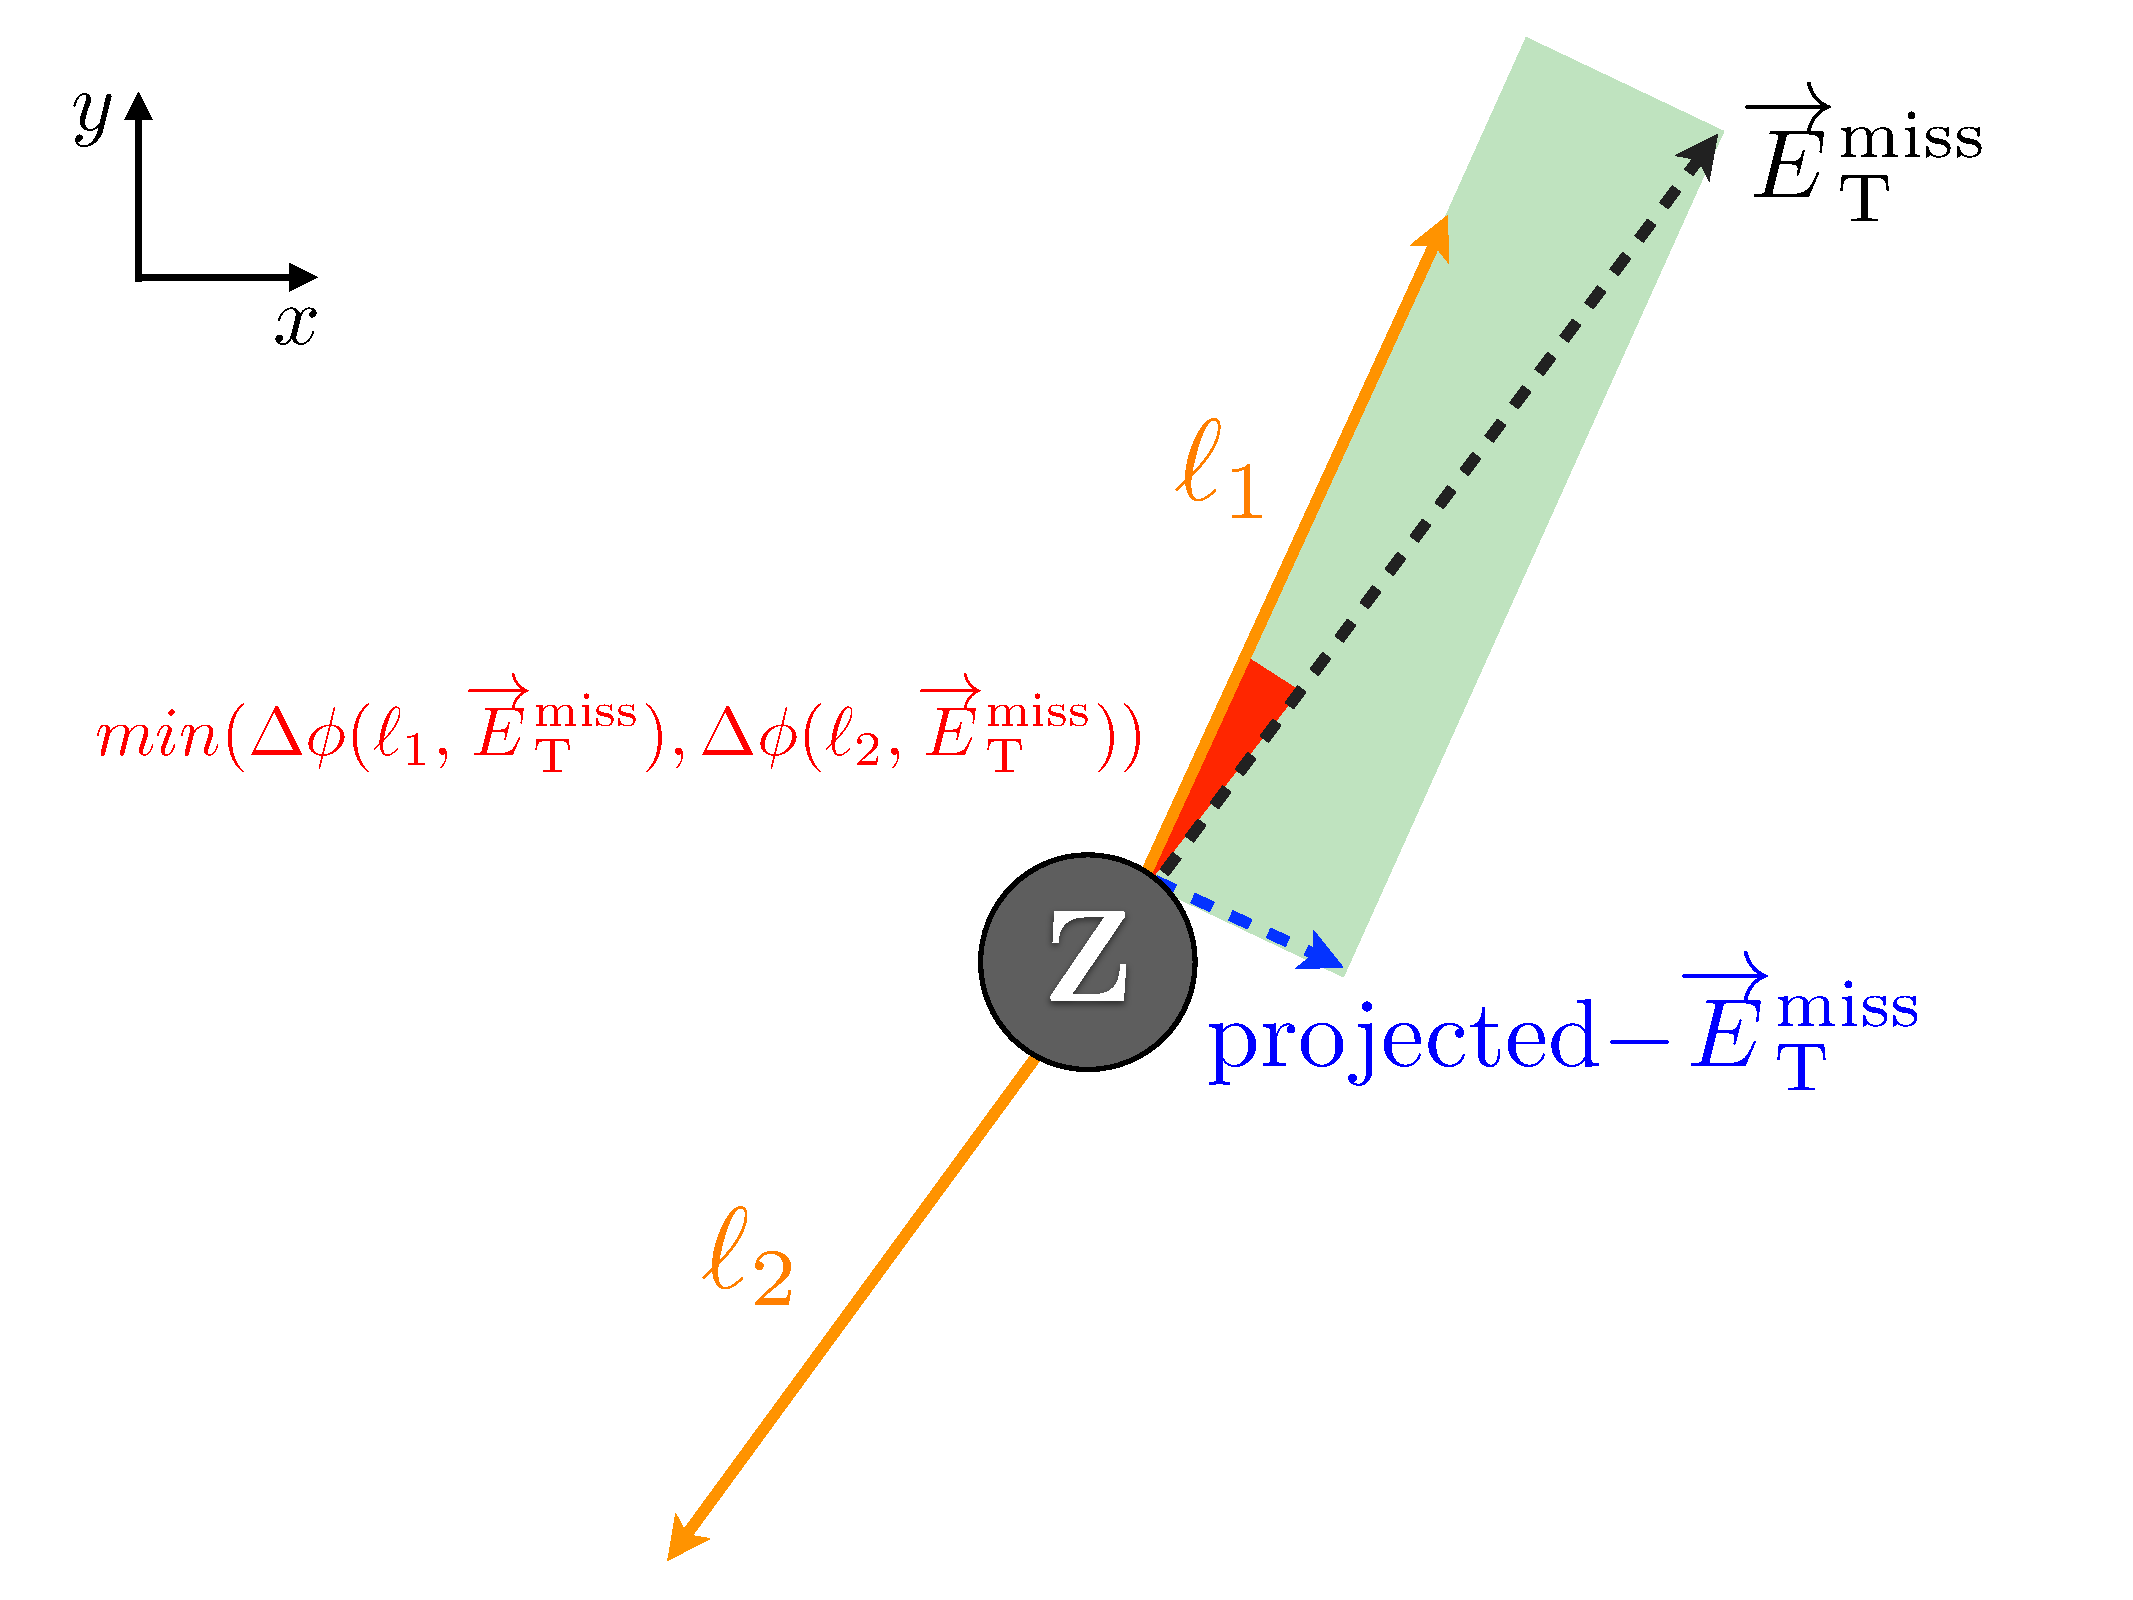
\includegraphics[width=0.7\textwidth]{figures/projmet.pdf} 
\end{tabular} 
\caption{Schematic of \pmet.}
\label{fig:projmetscheme} 
\end{figure}  
%
\begin{figure}[htp] 
\centering 
\begin{tabular}{c} 
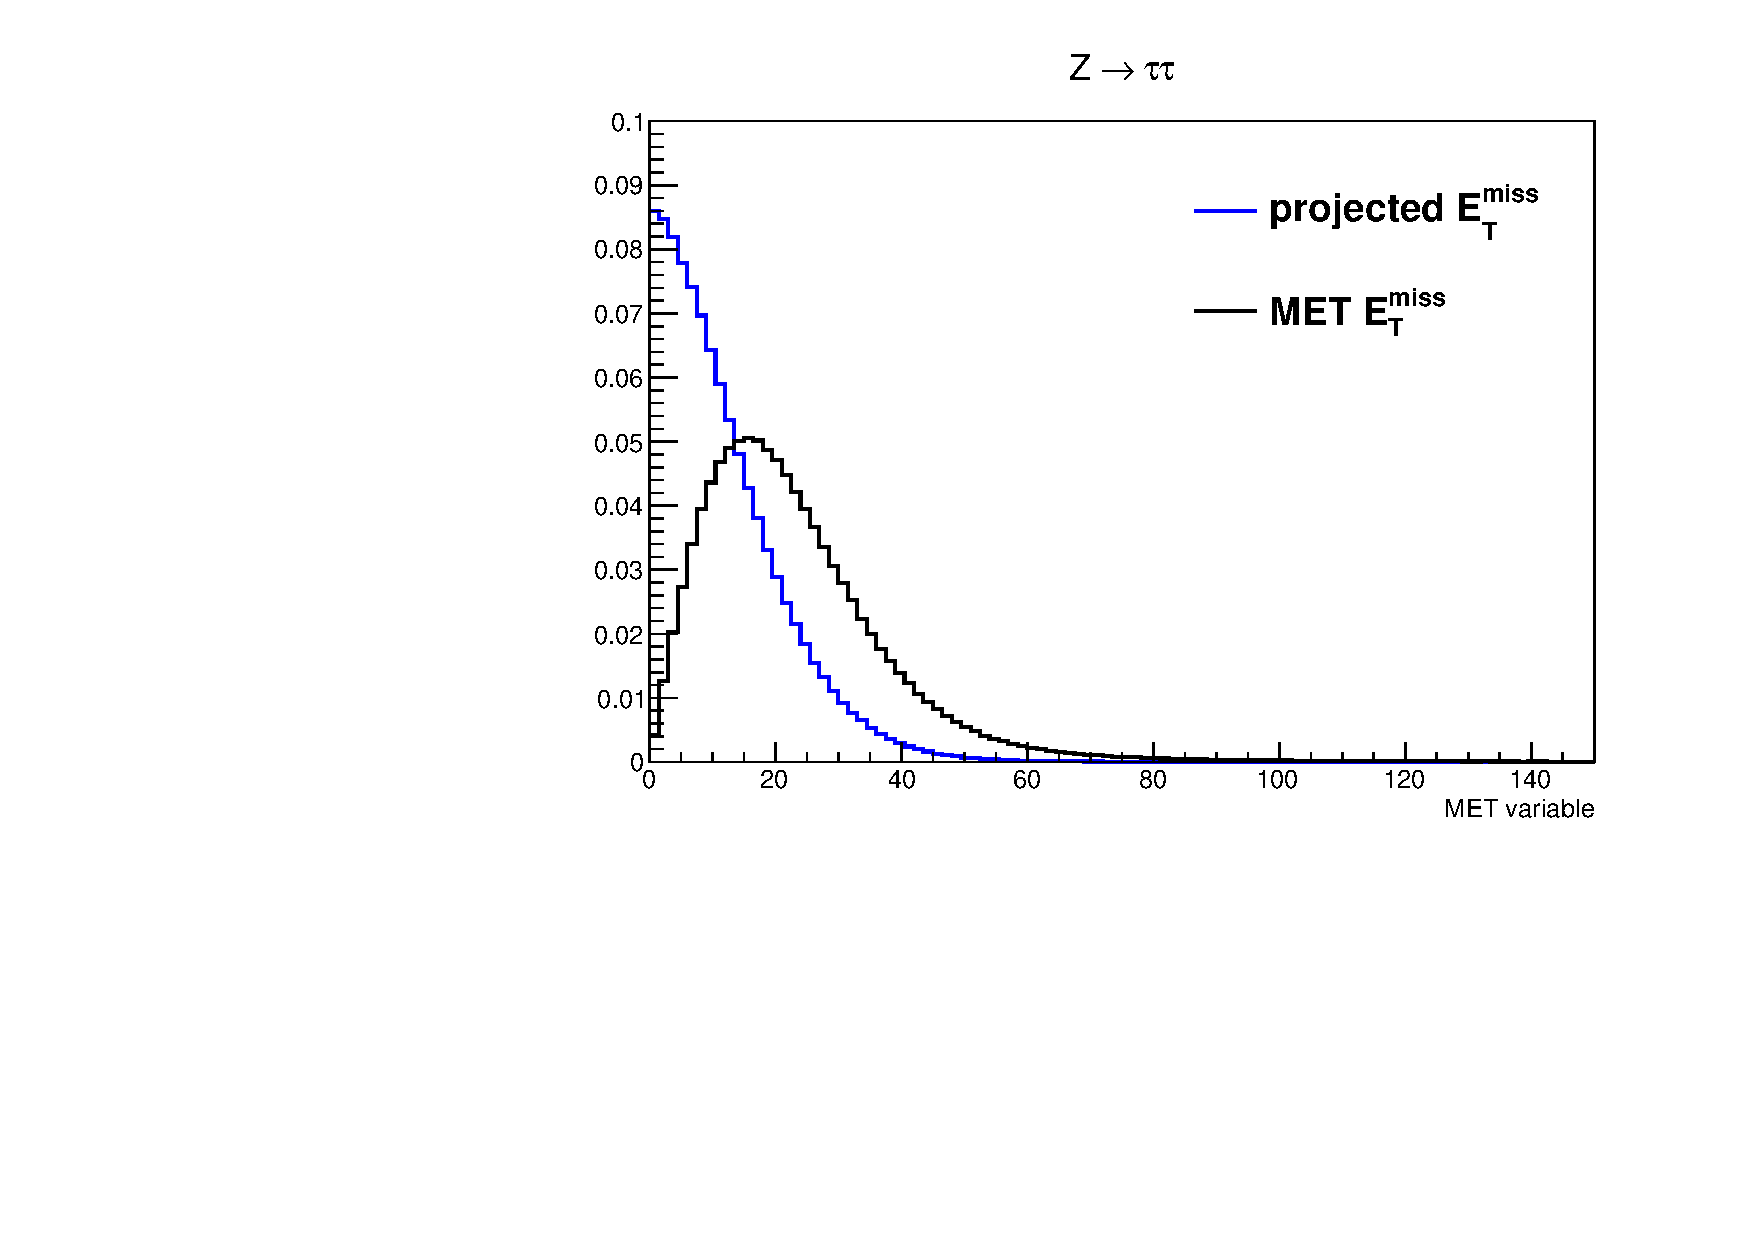
\includegraphics[width=0.45\textwidth]{figures/pmet_met_ztt.pdf} 
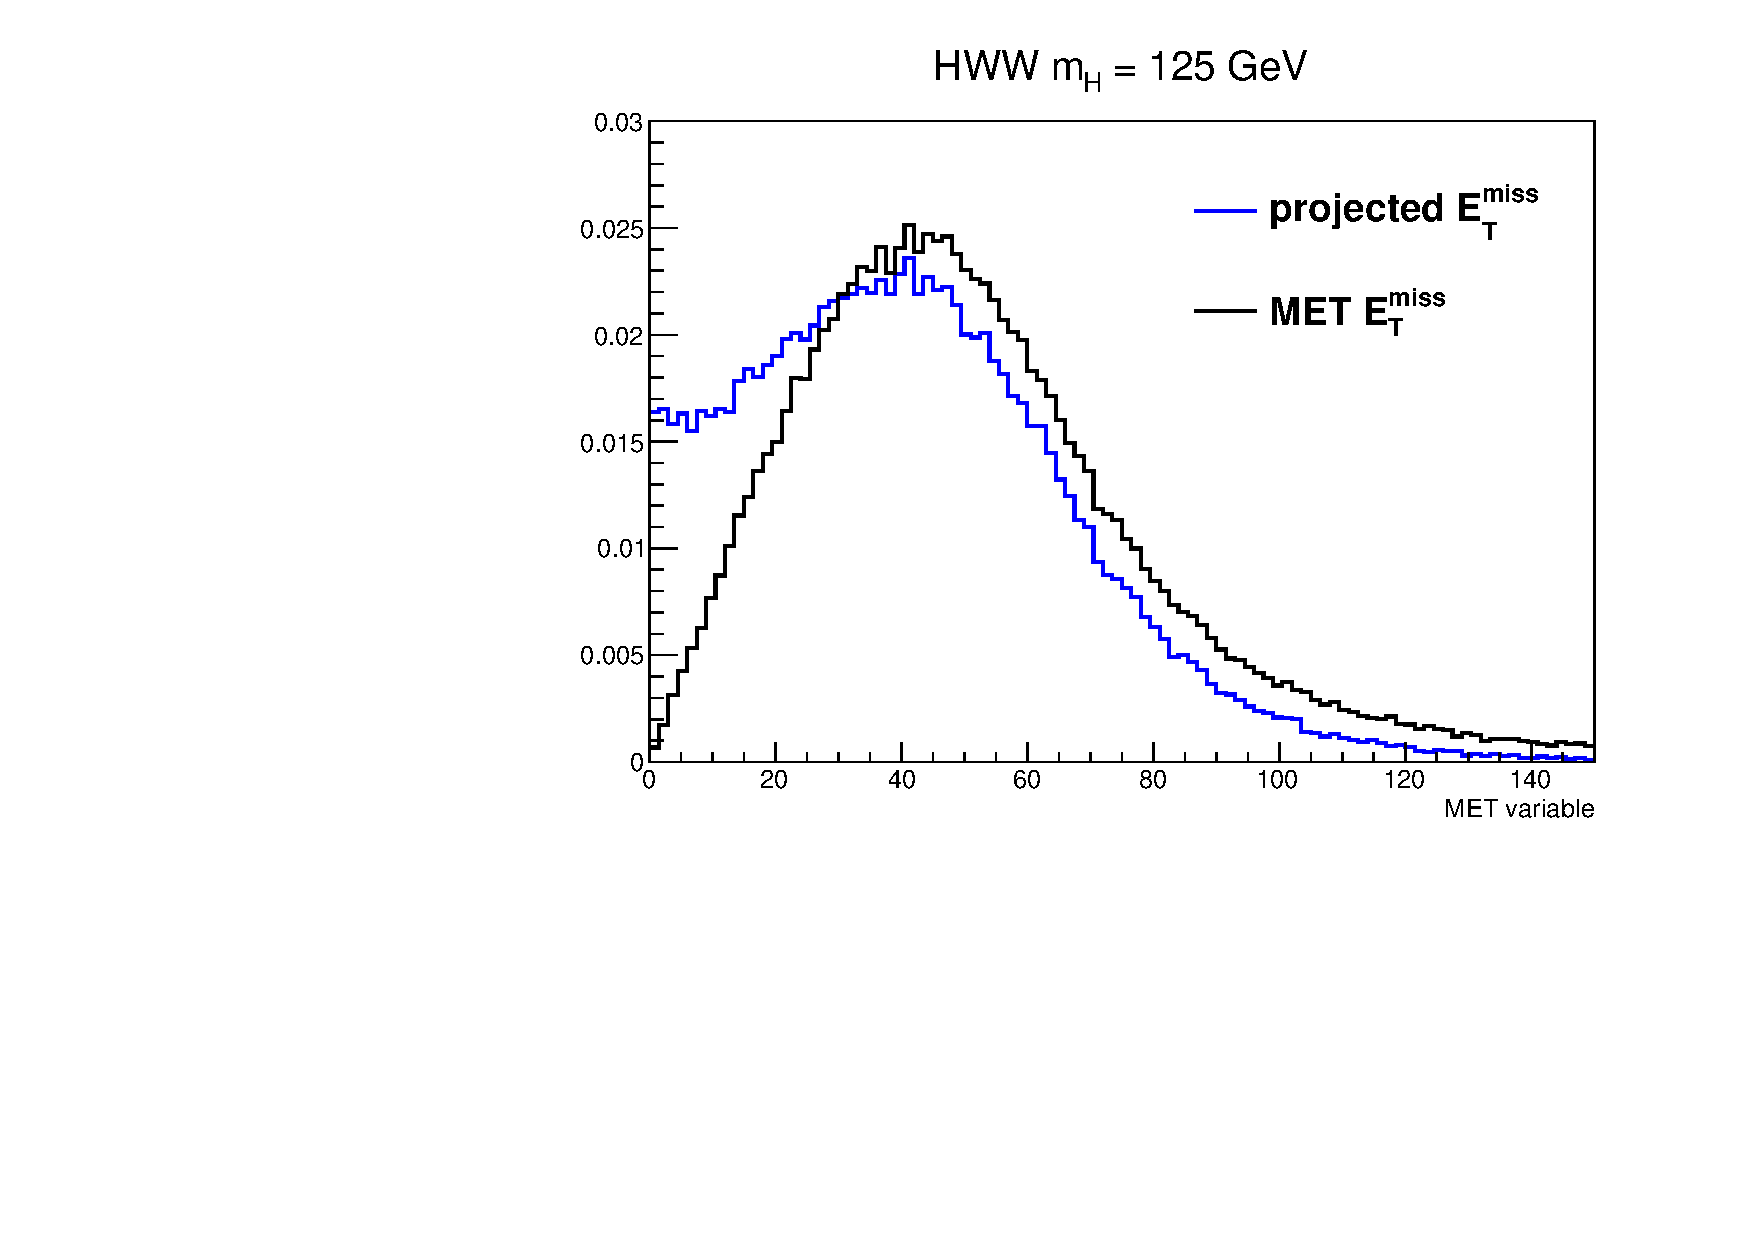
\includegraphics[width=0.45\textwidth]{figures/pmet_met_hww125.pdf} 
\end{tabular} 
\caption{\met(black) and \pmet(blue) in \dytt{}(left) and SM Higgs at \mHi=125~\GeV(right).}
\label{fig:projmet} 
\end{figure}  
Figure~\ref{fig:projmet} shows the \met{} and the \pmet{} distributions 
in black and red, repectively, in \dytt{} and SM Higgs at \mHi=125~\GeV\
on left and right, repectively. We can see that \pmet is more squeezed to 
the lower values in case of \dytt, giving better rejection power.  

The \trkmet\ is a variable insensitive to the pileup, 
but a drawback is that its tail is longer than \pfmet\ in the \dyll{} events. 
By isospin symmetry the average number of neutral hadrons should 
be same as that of the charged hadrons. But, if there is an imbalance between neutral 
and charged components in the jets, the \trkmet\ can be calculated arbitrarily high. 
For example, for a di-jet event with back-to-back 30~\GeV\ jets where one jet is composed 
of 10~\GeV\ of charged components and 20~\GeV\ of neutral components, and the other jet 
has the opposite composition, the \pfmet\ is 0 while \trkmet\ is 10~\GeV. 
Therefore, we use the minimum of \pfmet\ and \trkmet\, 
\begin{eqnarray} 
\minpmet = min \left( \pmet, \ptrkmet \right), 
\end{eqnarray} 
as a \met\ variable to protect \trkmet\ from those fluctuations. 
The other advantage of taking the minimum is that the the correlation 
between the two \met\ definitions is strong in the events with true \met, 
while weak in the events with fake \met\ as shown in Fig.~\ref{fig:2dmet}. 
So, by taking the minimum of them, we can get additional rejection 
of \dyll\ backgrounds without a harm to the signal.  
%
\begin{figure}[htp] 
\centering 
\begin{tabular}{c} 
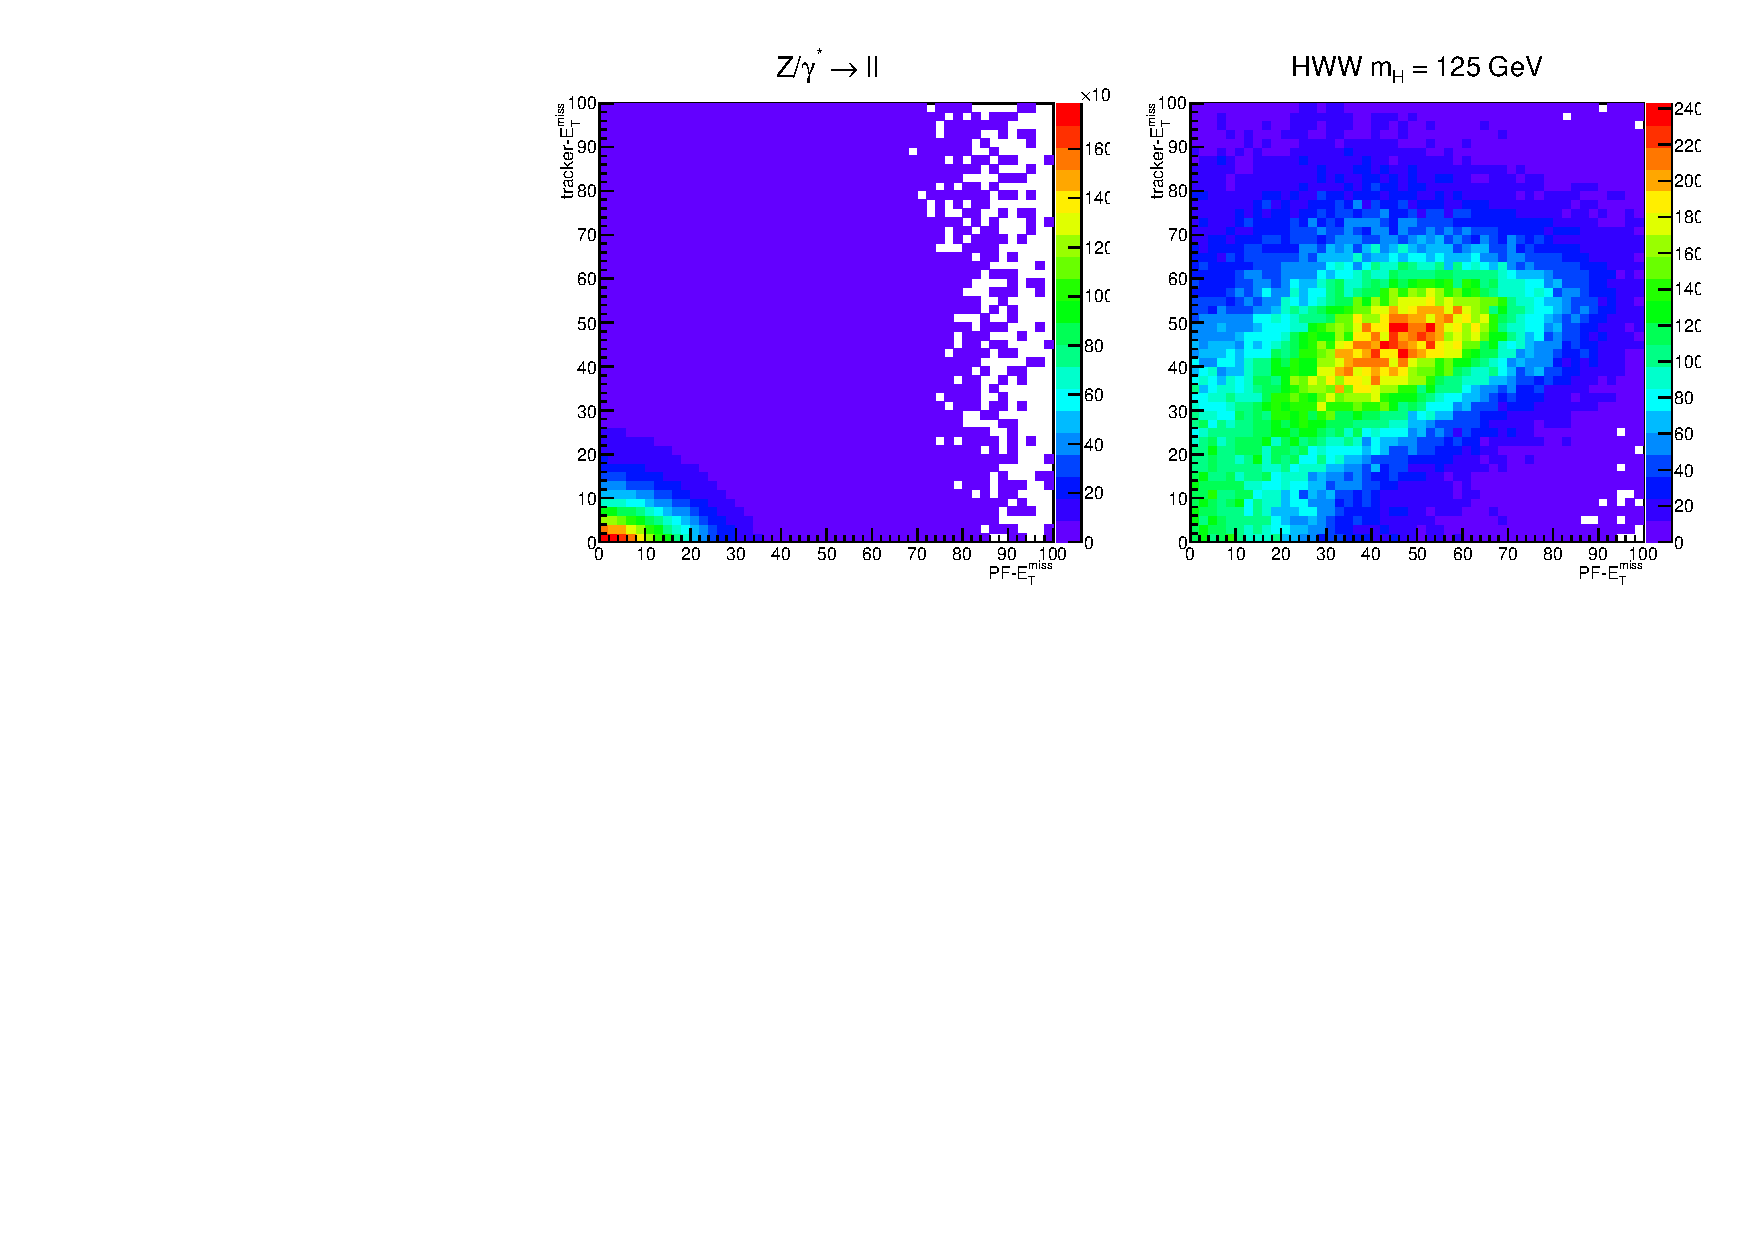
\includegraphics[width=0.99\textwidth]{figures/2dmet.pdf} 
\end{tabular} 
\caption{\pmet{} vs. \ptrkmet{} in \dyll{} and SM Higgs \mHi = 125~\GeV.}
\label{fig:2dmet} 
\end{figure}  

We require \minpmet{} to be greater than 20~\GeV\ in all categories as a baseline selecion. 
For further rejection of \dyll{} background, we apply MVA-based technique which will be 
discussed in detail in section~\ref{sec:dybkg}. 

%%%%%%%%%%%%%%%%%%%%%%%%%%%%%%%%%%%%%%%%%%%%%%%%%%%%%%%%%%%%%%%%%%
\section{ Top-tagging }
%\begin{itemize}
%\item \textcolor{red}{How B-tagging algorithm works and working point
%      (TCHEM : Track Counting High Efficiency Medium)}
%\item \textcolor{red}{how the discriminating variable is calculated }
%\item \textcolor{red}{quote some performance plots }
%\item \textcolor{red}{soft-muon tagging requirement }
%\end{itemize}

The \topbkg\ events contain additional b quarks on top of 
the two leptons and \met. The b quarks are then hadronized to B mesons, 
and develop hadronic showers. Experimentally,  
they can be identified by finding a displaced secondary vertex, B-tagging,
or a soft muon decayed from the B meson. 

The section~\ref{sec:btagging} described how the discriminator for b-tagging is constructed. 
If the b-tagging descriminator(TCHE) of a jet that passes 
the jet selection criteria described in section~\ref{sec:jetselection} 
is greater than 2.1, this jet is selected as a b-tagged jet. 
The event is rejected if there is at least one b-tagged jet. 
%\textcolor{red}{show MC vs Data of the discriminating variable in the top control region?}

We enhance the rejection of \topbkg{} backgrounds by removing events that contain 
non-isolated soft muons from heavy flavor decays. The following requirements are imposed to 
select soft muons. 
\begin{itemize} 
    \item $\pt > 3~\GeV$ 
    \item The muon should be a tracker muon
    \item The muon should have at least two muon segments one of which is 
          in the outermost muon station are matched.
    \item $N_{\textrm{track layers}}>5$ 
    \item $|d_{0}| < 0.2$~cm;
    \item $|d_{z}| <0.2$~cm;
    \item ${\rm{Iso}_{\textrm{Total}}}/{\pt}>0.1$ if $\pt>20~\GeV$.
\end{itemize} 
where $N_{\textrm{track layers}}$ is the number of tracker layers where the muon track has hits, 
$d_{0}$($d_{z}$) are the transverse(longitudinal) impact parameter with respect to 
the event primary vertex, and $\rm{Iso}_{\textrm{Total}}$ is the sum of \Et{} inside of the cone 
with $dR < 0.3$ in ECAL and HCAL, and \pt{} of tracker. Adding soft muon requirement 
especially helps in the 0-jet category where the top rejection efficiency increases 
about 50 \% compared to using b-tagging only.

The total top rejection efficiency using both methods when applied to \topbkg{} MC 
is about 50 \% in the 0-jet category and 80 \% in the 1-jet category. 


\section{\dyll\ suppression in \SF\ final states} 
\label{sec:dybkg}
%FIXME : I am here 
In the \SF\ channel, \dyll\ is one of the dominant backgrouds, 
and it is suppressed by rejecting events that have 
di-lepton mass around the Z mass. So, we veto events with 
$\left|\mll - \mZ \right| < 15~\GeV$. However, since the 
production rate of \dyll\ process is very large, even after
rejecting those events, there remains a significant contribution. 
To further reject this background, a tight \met\ requirement is typically imposed
because the \met\ in \dyll\ tends to be smaller than 
the \met\ in the signal process. 
This is because there is no genuine source of \met\ in the \dyll\ events. 
But, a strong \met\ selection can also lead to a significant loss in signal. 
So, we developed a BDT-based \dyll\ suppression technique~\cite{dymva} to recover the 
loss in the signal efficiency. 

The training is done with a combination of signal samples, \mHi = 125 and 200~\GeV, 
for signal and \dyll\ MC for background. The motivation of using a combination of the two 
\mHi\ points is to use one training for all \mHi\ points. The \DF\ events 
are used in the training because there should not be any difference in the training 
variables between \SF\ and \DF\ events. 
As a background sample, 
a combination of the Madgraph and the Powheg samples is used to maximize statistics. 
For the training, we apply the WW selection for the cut-based analysis
which is discussed in sec~\ref{sec:wwsel}.
The training is done separately in the 0-jet and 1-jet catagories. 

The input variables for the training are the following. 
\begin{itemize}

%
\item \met-related variables
\begin{itemize}
\item \pmet 
\item \ptrkmet  
\item \met\ significance : 
      $\displaystyle \frac{\met}{\sqrt{\sum_{i}^{\textrm{All objects}} E_T(i)}}$
      where $E_T(i)$ is the tranverse energy of the object i used for \met\ calculation
\end{itemize}

%
\item kinematic variables
\begin{itemize}
\item \ptll : di-lepton \pt 
\item \mT : Higgs transverse mass 
\item leading jet \pt
\item recoil of the di-lepton + \met\ system :     
      the magnitude of the vector sum of \pfmet\ and the di-lepton system 
\end{itemize}

%
\item azimuthal angle differences 
\begin{itemize}
\item $\Delta\phi(ll, \textrm{leading jet})$ : azimuthal angle difference between 
      the di-lepton system and the leading jet ($\pt>15~\GeV$)
\item $\Delta\phi(ll, \met)$ : azimuthal angle difference between the di-lepton system 
      and \met
\item $\Delta\phi(\textrm{leading jet}, \met)$ : azimuthal angle difference between 
      the leading jet ($\pt>15~\GeV$) and \met
\end{itemize}

%
\item other variable
\begin{itemize}
\item $N_{vtx}$ : number of reconstructed vertices 
\end{itemize}

\end{itemize}

\begin{figure}[htp] 
\centering
\begin{tabular}{c} 
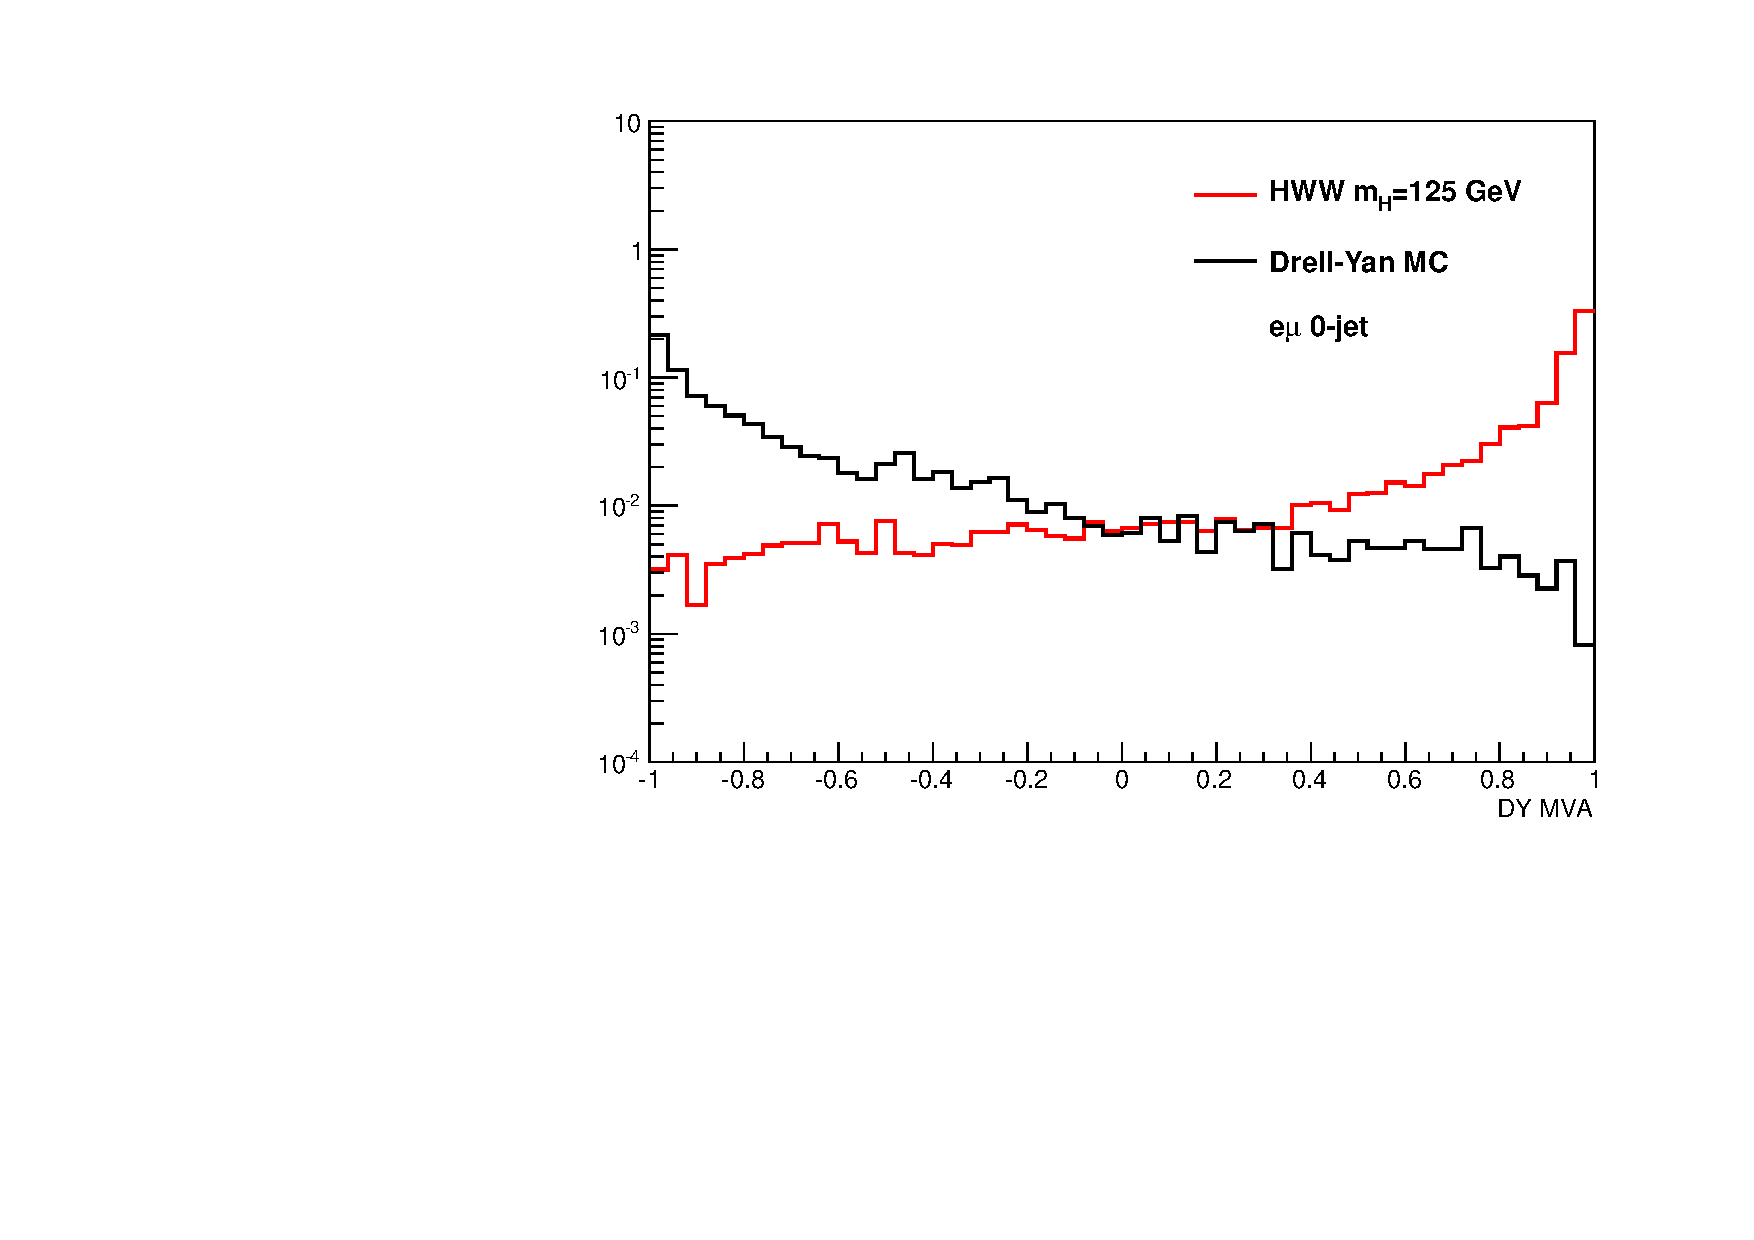
\includegraphics[width=0.5\textwidth]{figures/dymva_0j.pdf} 
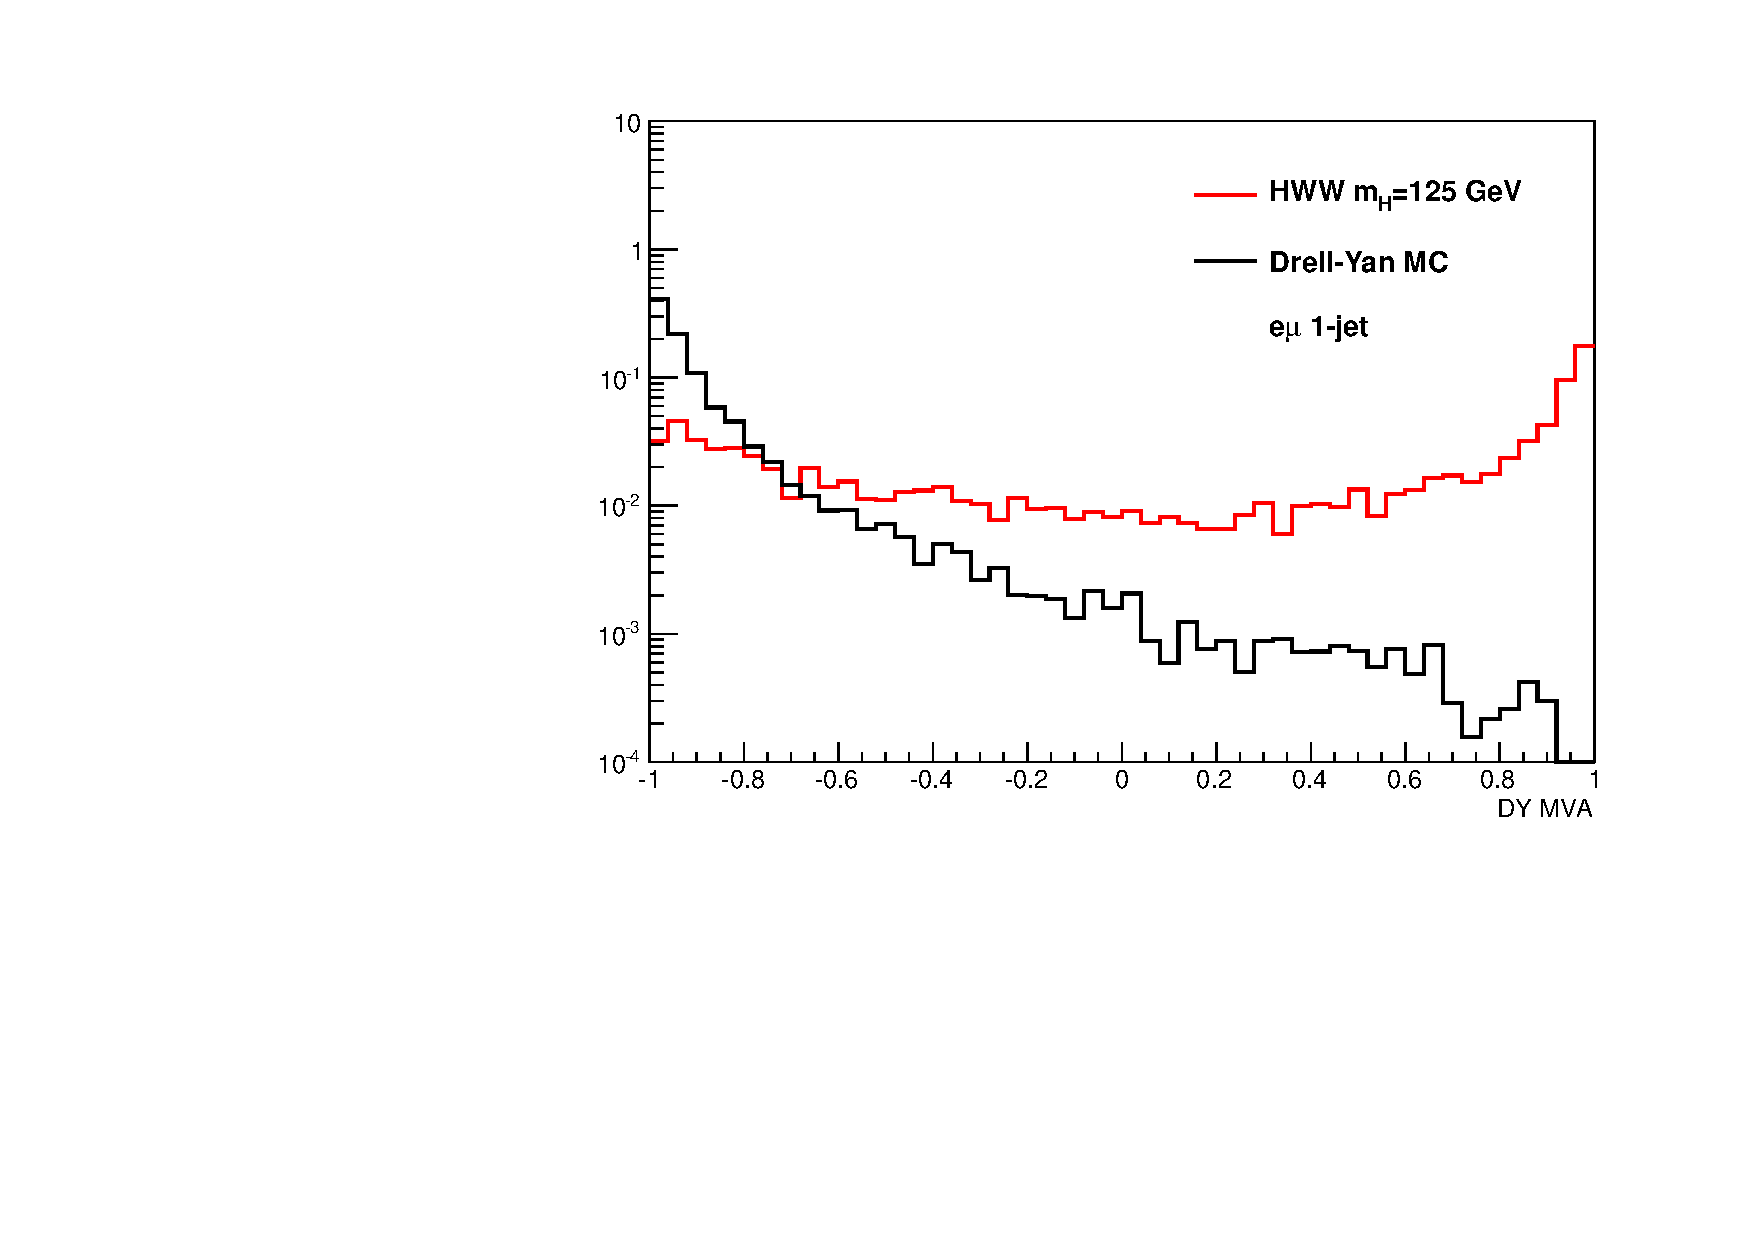
\includegraphics[width=0.5\textwidth]{figures/dymva_1j.pdf} 
\end{tabular} 
\caption{The BDT score for \mHi = 125~\GeV(red) and \dyll\ MC(black)
in 0-jet(left) and 1-jet(right) categories.} 
\label{fig:dymva} 
\end{figure} 

Figure~\ref{fig:dymva} shows the BDT scores for \mHi = 125~\GeV in red 
and \dyll\ MC in black in 0-jet(left) and 1-jet(right) categories. We finally require 
that the BDT score be greater than 0.88(0.84) in 0-jet(1-jet) category. 
This requirement is applied to only \SF\ category. 
The signal(\mHi=125~\GeV) efficiency of this selection is 50~\% and 35~\% 
in 0-jet and 1-jet categories, respectively, 
and the background(\dyll\ MC) efficieny is 0.5~\% and 0.1~\% in 0-jet and 1-jet categories
%The \DF\ category has only $\minpmet>20~\GeV$ requirement.

\section{Additional Selections}
When di-boson(\vv) events events with three or four leptons lose one or two leptons 
because they do not pass the lepton selection or flew out of the 
detector acceptance, they can pass the signal selection.  
To reject these contribution, we veto events if they contain 
a third lepton with $\pt>10~\GeV$. This requirement rejects about 30~\% of 
events containing more then two leptons in \vv. 

At low \mll\ region, there are multiple resonances such as 
$\Upsilon$($m_\Upsilon\sim 10~\GeV$) and $J/\psi$($m_{J/\psi}\sim 3~\GeV$).
In order to reject these resonances, we apply $\mll>12~\GeV$ . 

\Wjets\ background tends to have small \ptll\ because the lepton from W and 
the recoiling jet are likely to be back-to-back. So, in order to suppress 
\Wjets\ further, $\ptll>30(45)~\GeV$ is applied for shape-based (cut-based) apporoaches. 

\section{WW Selection}
\label{sec:wwsel}
All requirements imposed so far are designed to select events containing 
a pair of W. This baseline selection is called ``WW selection" and 
the stage of selection where the WW selection is applied is called ``WW level".
By applying WW selection, we can reach better signal-to-background ratio(S/B),
therefore a reasonable extraction of signal becomes possible. 
Table~\ref{tab:wwselection} summarizes the requirements of the WW selection. 

\begin{table}[htp] 
\begin{center} 
\begin{tabular}{c|cc}
\hline
Selection & \DF & \SF \\
\hline \hline 
\ptlmax & $>20~\GeV$ & $>20~\GeV$ \\
\ptlmin & $>10~\GeV$ & $>10~\GeV$ \\
Lepton selection & applied & applied \\
Number of jet selection & applied & applied \\
Third lepton veto & applied & applied \\
opposite-sign requirement & applied & applied \\
\mll & $>12~\GeV$ & $>12~\GeV$ \\
$\left| \mll - m_Z \right| > 15~\GeV$ & not applied & applied \\
\minpmet & $>20~\GeV$ & $>20~\GeV$ \\
BDT-based Drell-Yan suppression & not applied & applied \\
Top veto & applied & applied \\
\ptll & $>30~\GeV$[*] & $>45~\GeV$ \\
\hline
\end{tabular} 
\caption{Summary of WW selection. [*] For shape-based method 
$\ptll>30~\GeV$ is applied and for cut-based method $\ptll>45~\GeV$ is applied.}
\label{tab:wwselection} 
\end{center} 
\end{table} 


